\documentclass[DynamicalBook]{subfiles}
\begin{document}
%




\setcounter{chapter}{0}%Just finished 0.


%------------ Chapter ------------%
\chapter{Deterministic Systems}\label{chapter.1}

\section{Introduction}

Here's a basic fact of life: \emph{things change}. And how things change most
often depends on how they currently are. This is the basic idea underlying all the various notions of \emph{dynamical
  system} that we will see in this book.

\begin{informal}
  A \emph{dynamical system} consists of:
  \begin{itemize}
  \item a notion of how things are, called the \emph{state}, and
  \item a notion of how things will change given how they are, called the \emph{dynamics}.
  \end{itemize}
  The dynamics of a system might also depend on some free \emph{parameters}, and
  we will often only be interested in some particular \emph{variables} of the
  state. 
\end{informal}

In this chapter, we will see this idea in its
most distilled form: we will know exactly how things are, and what they will be
like next. That is, we'll be focusing on \emph{deterministic} dynamical systems,
whose time steps forward in \emph{discrete} increments.


A paradigmatic example of this sort of dynamical system is a clock.
\[
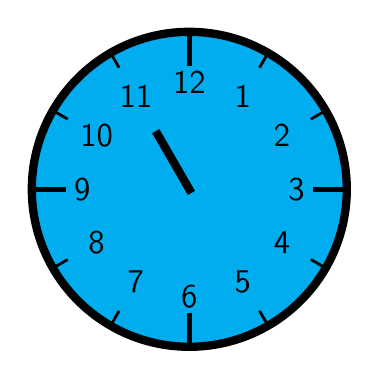
\begin{tikzpicture}[line cap=rect,line width=3pt]
\filldraw [fill=cyan] (0,0) circle [radius=2cm];
\foreach \angle [count=\xi] in {60,30,...,-270}
{
  \draw[line width=1pt] (\angle:1.8cm) -- (\angle:2cm);
  \node[font=\large] at (\angle:1.36cm) {\textsf{\xi}};
}
\foreach \angle in {0,90,180,270}
  \draw[line width=2pt] (\angle:1.6cm) -- (\angle:2cm);
\draw (0,0) -- (120:0.8cm);
\end{tikzpicture}
\]

Suppose that our clock has just an hour hand for now. Then we may collect all
the way things can be for the clock into a set of hours:
$$\Set{Hours} := \{1, 2, 3, 4, 5, 6, 7, 8, 9, 10, 11, 12\}.$$

The set $\Set{Hours}$ is the set of \emph{states} of our clock system. If we know what hour it is, we also know what hour is coming next. So, this system has the following dynamics:
%
% :CUSTOM-ID: problem-with-drawing-mapsto-nicely
%
\begin{align*}
  \fun{tick} : \Set{Hours} &\to \Set{Hours} \\
                t &\mapsto \begin{cases} t + 1 &\mbox{if $t < 12$}\\ 1 &\mbox{if $t = 12$}  \end{cases}
\end{align*}

Here's a sample of the dynamics of the clock. Say we started at 3 o'clock:
$$3 \xmapsto{\fun{tick}} 4 \xmapsto{\fun{tick}} 5 \xmapsto{\fun{tick}} 6
\xmapsto{\fun{tick}} \cdots$$

Not the most dynamic of systems, but we have to start somewhere. If we want to
refer to the whole system at once, we can box it up and write it like this:

\begin{equation}\label{eqn.clock_system_box}
\begin{tikzpicture}[oriented WD, every fit/.style={inner xsep=\bbx, inner ysep=\bby}, bbx = 1cm, bby =.5cm, bb min width=1cm, bb port length=4pt, bb port sep=1, baseline=(X.center)]
	\node[bb={0}{1}] (X) {$\Sys{Clock}$};
	\draw[label] 
		node [right=2pt of X_out1] {$\Set{Hours}$}
		;
\end{tikzpicture}
\end{equation}

We imagine that the clock is going about its business inside the box, and
that is shows the hour it is currently displaying on the outgoing wire.

One issue with our clock is that it doesn't tell us whether it is morning or
evening. Being morning or evening is its own way that things might be, and we
can see it as its own dynamical system. We might imagine a little addition to
our clock that reads $\const{a.m.}$ or $\const{p.m.}$:
\[
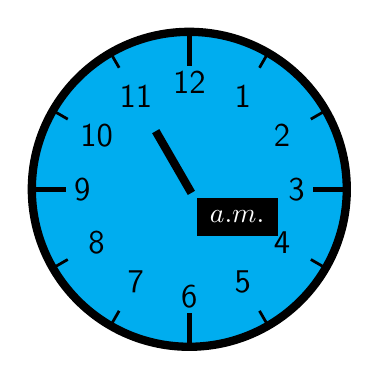
\begin{tikzpicture}[line cap=rect,line width=3pt, baseline=(bl)]
\coordinate (bl) at (0,0);
\filldraw [fill=cyan] (0,0) circle [radius=2cm];
\foreach \angle [count=\xi] in {60,30,...,-270}
{
  \draw[line width=1pt] (\angle:1.8cm) -- (\angle:2cm);
  \node[font=\large] at (\angle:1.36cm) {\textsf{\xi}};
}
\foreach \angle in {0,90,180,270}
  \draw[line width=2pt] (\angle:1.6cm) -- (\angle:2cm);
\draw (0,0) -- (120:0.8cm);
\node[draw, fill] at (330:.7cm) {${ \color{white}\const{a.m.} }$};
\end{tikzpicture}
\]

We can see this little addition as a system in its own right; it is the system
of $\const{a.m.}/\const{p.m.}$. The states of this system are
$$\Set{Meridien} = \{\const{a.m.}, \const{p.m.}\}.$$
But this time, knowing how they are going to change also requires us to know the
hour:
\begin{align*}
  \fun{next} : \Set{Meridien} \times \Set{Hours} &\to \Set{Meridien} \\
               (\const{a.m.}, t) &\mapsto \begin{cases} \const{p.m.} &\mbox{if $t = 11$}\\ \const{a.m.} &\mbox{otherwise}  \end{cases} \\
               (\const{p.m.}, t) &\mapsto \begin{cases} \const{a.m.} &\mbox{if $t = 11$}\\ \const{p.m.} &\mbox{otherwise}  \end{cases}
\end{align*}
If it is $\const{a.m.}$ and the clock reads 8, then it will still be
$\const{a.m.}$; but if it is $\const{a.m.}$ and the clock reads 11, then it will
switch on the next hour to $\const{p.m.}$.

The thing to note about the dynamics of the $\const{a.m.}/\const{p.m.}$ system
is that they depend on what hour it is. The hour is a \emph{parameter} for the
dynamics of this system. We can draw this system as a box like this:
\begin{equation}\label{eqn.am_pm_system_box}
\begin{tikzpicture}[oriented WD, every fit/.style={inner xsep=\bbx, inner ysep=\bby}, bbx = 1cm, bby =.5cm, bb min width=1cm, bb port length=4pt, bb port sep=1, baseline=(X.center)]
	\node[bb={1}{1}] (X) {$\Sys{a.m./p.m.}$};
	\draw[label] 
		node [left=2pt of X_in1] {$\Set{Hours}$}
		node [right=2pt of X_out1] {$\Set{Meridien}$}
		;
\end{tikzpicture}
\end{equation}
We have the $\Set{Meridien}$ wire coming out, which carries the information of
whether it is $\const{a.m.}$ or $\const{p.m.}$, just like the clock. But we also
have a wire coming in, which carries the hour that we need as a parameter for
our dynamics.


We can now express our whole clock (\ref{eqn.whole_clock}) by wiring together
our bare clock and the $\const{a.m.}/\const{p.m.}$ system:

\begin{equation}\label{eqn.whole_clock_system_box}
\begin{tikzpicture}[oriented WD, every fit/.style={inner xsep=\bbx, inner ysep=\bby}, bbx = .3cm, bby =.3cm, bb min width=.5cm, bb port length=2pt, bb port sep=1, baseline=(Y.center)]
	\node[bb={1}{1}] (X1) {$\Sys{a.m./p.m.}$};
  	\node[bb={0}{1}, below=2 of X1] (X2) {$\Sys{Clock}$};
	\node[bb={0}{2}, fit={($(X1.north west)+(-2,1)$) ($(X1.north east)+(2,1)$) ($(X2.south)+(0,-3)$)}] (Y) {};
  \node[above=0pt of Y.south] (Label) {$\Sys{ClockWithDisplay}$};
	\draw (X1_out1) to (Y_out1);
  \draw let \p1=(X1.south west), \p2=(X2.north east), \n1=\bbportlen, \n2=\bby in
    (X2_out1) to[in=0] (\x2 + \n1, \y2 + \n2) -- (\x1 - \n1, \y2 + \n2) to[out=180] (X1_in1);
  \draw (X2_out1) to (Y_out2);
	\draw[label] 
		node [right=2pt of Y_out1] {$\Set{Meridien}$}
		node [right=2pt of Y_out2] {$\Set{Hours}$}
		;
\end{tikzpicture}
\end{equation}

This system has states
$$\Set{HoursWithDisplay} := \Set{Hours} \times \Set{Meridien}$$
consisting of a pair $(11, \const{a.m.})$ of an hour and a meridien reading.
They update in a combined way, by using the hour shown on the clock face as the
parameter we need for the $\const{a.m.}/\const{p.m.}$ system. In full, the
dynamics looks like this:
\begin{align*}
  \fun{tick'} :\Set{HoursWithDisplay} &\to \Set{HoursWithDisplay} \\
  (t, m) &\mapsto (\fun{tick}(t), \fun{next}(t, m))
\end{align*}

\begin{exercise}
  Expand the definition of the combined system out in full, and check that it
  really does behave like the clock with $\const{a.m.}/\const{p.m.}$ display should.
\end{exercise}

Now that we have a working clock, we can use it for systems that need to know
the time. For example, consider a diner that opens at $7 \const{a.m.}$ and
closes at $10 \const{p.m.}$. The states of this diner are
$$\Set{DinerState} = \{\const{open}, \const{closed}\}.$$
The diner's dynamics are then
\begin{align*}
  \fun{dinerDynamics} : \Set{DinerState} \times \Set{HoursWithDisplay} &\to \Set{DinerState} \\
  (\const{open}, (10, \const{p.m.})) &\mapsto \const{closed} \\
  (\const{closed}, (7, \const{a.m.})) &\mapsto \const{open} \\
  (s, (t, m)) &\mapsto s \quad\mbox{otherwise.} 
\end{align*}

Again, we can represent the diner by this box:
\begin{equation}\label{eqn.diner_system_box}
\begin{tikzpicture}[oriented WD, every fit/.style={inner xsep=\bbx, inner ysep=\bby}, bbx = 1cm, bby =.5cm, bb min width=1cm, bb port length=4pt, bb port sep=1, baseline=(X.center)]
	\node[bb={2}{1}] (X) {$\Sys{Diner}$};
	\draw[label] 
		node [left=2pt of X_in1] {$\Set{Meridien}$}
		node [left=2pt of X_in2] {$\Set{Hours}$}
		node [right=2pt of X_out1] {$\Set{DinerState}$}
		;
\end{tikzpicture}
\end{equation}
This time, we have two wires coming in, corresponding to the two parameters we
need for the diner system: the hour and the
meridien. 

Assuming that the diner has a clock on its wall which it uses to decide whether
to open or close, the full diner system would be given by wiring the clock with display into
those input wires:
\begin{equation}\label{eqn.diner_system_box}
\begin{tikzpicture}[oriented WD, every fit/.style={inner xsep=\bbx, inner ysep=\bby}, bbx = 1cm, bby =.5cm, bb min width=1cm, bb port length=4pt, bb port sep=1, baseline=(Outer.center)]
  \node[bb={0}{2}](Clock) {$\Sys{ClockWithDisplay}$};
  \node[bb={2}{1}, right=of Clock] (Diner) {$\Sys{Diner}$};
  
  \node[bb={0}{1}, fit={(Clock) (Diner)}] (Outer) {};

  \draw (Clock_out1) to (Diner_in1);
  \draw (Clock_out2) to (Diner_in2);
  \draw (Diner_out1) to (Outer_out1);

  \draw[label] node [right=2pt of Outer_out1] {$\Set{DinerState}$};
\end{tikzpicture}
\end{equation}
If we want to, we can peak into the clock with display and see that it is itself
made out of a clock wired to a display:
\begin{equation}\label{eqn.diner_system_box}
\begin{tikzpicture}[oriented WD, every fit/.style={inner xsep=\bbx, inner ysep=\bby}, bbx = 1cm, bby =.3cm, bb min width=1cm, bb port length=4pt, bb port sep=1, baseline=(Outer.center)]
	\node[bb={1}{1}] (X1) {$\Sys{a.m./p.m.}$};
  	\node[bb={0}{1}, below=2 of X1] (X2) {$\Sys{Clock}$};
	\node[dashed, bb={0}{2}, fit={($(X1.north west)+(0,1)$) ($(X1.north east)+(0,1)$) ($(X2.south)+(0,-3)$)}] (Clock) {};
  \node[above=0pt of Clock.south] (Label) {$\Sys{ClockWithDisplay}$};
	\draw (X1_out1) to (Clock_out1);
  \draw let \p1=(X1.south west), \p2=(X2.north east), \n1=\bbportlen, \n2=\bby in
    (X2_out1) to[in=0] (\x2 + \n1, \y2 + \n2) -- (\x1 - \n1, \y2 + \n2) to[out=180] (X1_in1);
  \draw (X2_out1) to (Clock_out2);
  \node[bb={2}{1}, right=of Clock] (Diner) {$\Sys{Diner}$};
  
  \node[bb={0}{1}, fit={(Clock) (Diner)}] (Outer) {};

  \draw (Clock_out1) to (Diner_in1);
  \draw (Clock_out2) to (Diner_in2);
  \draw (Diner_out1) to (Outer_out1);

  \draw[label] node [right=2pt of Outer_out1] {$\Set{DinerState}$};
\end{tikzpicture}
\end{equation}

These examples are simple, but it doesn't take much more to get to some truly
amazing phenomena. Consider this system: we have an infinite tape with a
read-head at some position. On this infinite tape, we will write the symbols
$a$, $b$, $c$, or $d$, or we will leave it blank: $\_$. Together, the state
of the tape and the position of the read-head have states pairs $(\fun{T}, n)$ of a
function $\fun{T} : \zz \to \{a, b,c,d\_\}$ telling us what symbol $\fun{T}(i)$ is drawn at
position $i$ of the tape, and the position $n$ of the read-head:
\begin{align*}
  \Set{Symbol} &= \{a, b,c,d\_\}
  \Set{Tape} &= \Set{Symbol}^{\zz}\\
  \Set{Head} &= \zz
\end{align*}
The way this system can change is by reading in a move command and a
write command. The move command will be either move left, a command of $-1$, or
move right, a command of $1$:
$\Set{Move} = \{-1, 1\}$. The write command will be one of the
symbols that can be written on the tape: $\Set{Write} = \{0, 1,2,3\_\}$.

The way this system changes is by writing the write command to the tape at that
position, and then moving according to the move command. As a function, this is:
\begin{align*}
  \fun{execute} : \Set{Tape} \times \Set{Head} \times \Set{Move} \times \Set{Write} &\to \Set{Tape} \Set{Head} \\
  ((\fun{T}, n), d, s) &\mapsto \left( i \mapsto \begin{cases} \fun{T}(i) &\mbox{if $i \neq n$} \\ s &\mbox{if $i = n$} \end{cases},\, n + d \right)
\end{align*}

We can imagine that the system shows tape and the symbol under the read head. We can box this system up like so:
\begin{equation}\label{eqn.turing_box}
\begin{tikzpicture}[oriented WD, every fit/.style={inner xsep=\bbx, inner ysep=\bby}, bbx = 1cm, bby =.5cm, bb min width=1cm, bb port length=4pt, bb port sep=1, baseline=(Tape.center)]
\node[bb={2}{2}] (Tape) {$\Sys{Tape Machine}$};
\draw[label]
  node[left=2pt of Tape_in1] {$\Set{Move}$}
  node[left=2pt of Tape_in2] {$\Set{Write}$}
  node[right=2pt of Tape_out1] {$\Set{Tape}$}
  node[right=2pt of Tape_out2] {$\Set{Symbol}$}
;
\end{tikzpicture}
\end{equation}

Now, we need one more simple ingredient to get our system going; a mysterious system of the
form:
\begin{equation}\label{eqn.turing_box2}
\begin{tikzpicture}[oriented WD, every fit/.style={inner xsep=\bbx, inner ysep=\bby}, bbx = 1cm, bby =.5cm, bb min width=1cm, bb port length=4pt, bb port sep=1, baseline=(Box.center)]
\node[bb={1}{2}] (Box) {$\Sys{Mystery Box}$};
\draw[label]
  node[right=2pt of Box_out1] {$\Set{Move}$}
  node[right=2pt of Box_out2] {$\Set{Write}$}
  node[left=2pt of Box_in1] {$\Set{Symbol}$}
;
\end{tikzpicture}
\end{equation}

We can see that our mystery box will take in a symbol and put out a move command
and a write command. The way our mystery box behaves is rather mysterious: here it is in a table,
where the entry in the row $i$ and the column $s$ is written $(m,w):s'$ for the
move command $m$, the write command $w$, and the next state $s'$ that our
mysterious sytem transitions to when input the symbol $i$ in state $s$:
\begin{equation}\label{eqn.turing_machine}
  \begin{tabular}{|c|c|c|c|c|c|c|}
    \hline
     & 1 & 2 & 3 & 4 & 5 & 6 \\\hline
    a & (-1, b):1 & (1, a):1 & (-1, b):3  & (1, b):2 & (-1, b):6 & (-1, b):4 \\\hline     
   b & (-1, a):1 & (1, a):2 & (-1, b):5  & (1, a):4 & (1, a):6 & (1, a): 5 \\\hline     
   c & (1, d):2 & (1, d):2 & (-1, c):5 & (1,d):4 & (1, c):5 & (1, a):1 \\\hline     
   d & (-1, c):1 & (1, a):5 & (-1, c):3 & (1,d):5 & (-1, b):3 & end \\\hline     
  \end{tabular}
\end{equation}
Mysterious in deed. But when we wire the two together, magic happens!

\begin{equation}\label{eqn.full_turing_machine}
\begin{tikzpicture}[oriented WD, every fit/.style={inner xsep=\bbx, inner ysep=\bby}, bbx = 1cm, bby =.5cm, bb min width=1cm, bb port length=2pt, bb port sep=1, baseline=(Outer.center)]
  \node[bb={1}{2}](Box) {$\Sys{Mystery Box}$};
  \node[bb={2}{2}, right=of Box] (Tape) {$\Sys{Tape Machine}$};
  
  \node[bb={0}{0}, fit={($(Tape.south east) + (0, -2)$) ($(Box.north west) + (0, 1)$)}] (Outer) {};
  \node[above=0pt of Outer.south] (Label) {$\Sys{Universal Turing Machine}$};

  \draw (Box_out1) to (Tape_in1);
  \draw (Box_out2) to (Tape_in2);

  \draw (Tape_out1) to (Outer.east|-Tape_out1);
  \draw (Tape_out2) to (Outer.east|-Tape_out2);

  \draw let \p1=(Tape.south east), \p2=(Box.south west), \n1=\bbportlen, \n2=\bby in
    (Tape_out2) to[in=0] (\x1 + \n1, \y1 - \n2 - 1) -- (\x2 - \n1, \y2 - \n2 - 1) to[out=180] (Box_in1);
\end{tikzpicture}
\end{equation}
This is a universal Turing machine, capable of arbitrarily complex calculation
(if we encode everything into this strange alphabet)! Even small systems can
have very interesting behavior when plugged in to the right environment''.

%%
%% :CUSTOM_ID:cite-this.turing_machine
%% 

We call this way of putting together dynamical systems to make more complex
systems \emph{composition}.
\begin{informal}
  \emph{Composition} is the process by which some things are brought together to
  form bigger things.

  Functions can be composed by $g \circ f(x) = g(f(x))$, and dynamical systems
  can be composed by plugging in the variables of the states of some into the
  parameters of others.
\end{informal}

This book is all about composing dynamical systems. Because of this, we will use
the abstract language of composition: \emph{category theory}.
\begin{informal}
\emph{Category theory} is the abstract study of composition.
\end{informal}



\subsection{Category Theory}

We'll be using the language of category theory quite freely in this book, and so
we'll expect you to know the basics. These are the notions we will expect you to
be familiar with:
\begin{itemize}
\item What a category is.
\item What an isomorphism is.
\item What a functor is.
\item What a natural transformation is.
\item What a terminal and an initial object are.
\item What a product and a coproduct are.
\item What a monad is, and it will help if you also know what a comomad is.
  \item What a monoidal category is.
\end{itemize}

Good introductions to category theory abound. One place to start is \emph{Seven
  Sketches: An invitation to applied category theory}.

We will be using cartesian categories quite a bit in the first few chapters.
\begin{definition}\label{def.cartesian_category}
  A category $\cat{C}$ is \emph{cartesian} if every two objects $A$ and $B$ in
  $\cat{C}$ have a product $A \times B$, and $\cat{C}$ has a terminal object
  $\ord{1}$. Equivalently, $\cat{C}$ is cartesian if for any finite set $I$ and
  $I$-indexed family $A_{(-)} : I \to \cat{C}$ of objects, there is a product
  $\prod_{i \in I} A_i$ in $\cat{C}$.

  A functor $F : \cat{C} \to \cat{D}$ between cartesian categories is said to be
  \emph{cartesian} if the
  map $(F\pi_A,\, F\pi_B) : F(A \times B) \to FA \times FB$ is an isomorphism
  for all $A$ and $B$, and the terminal morphism $F\ord{1} \to \ord{1}$ is an
  isomorphism. 
\end{definition}

We will also use some more advanced category theory, like indexed
categories, double categories, and toposes. But we will introduce these concepts
as we use them.
\section{Deterministic Systems}

That's a lot of informal definitions, we are ready for something precise:
\begin{definition}\label{def.deterministic_system}
  A \emph{deterministic system} $\Sys{S}$, also written as $$\lens{\update{S}}{\expose{S}} : \lens{\State{S}}{\State{S}} \leftrightarrows \lens{\In{S}}{\Out{S}},$$ consists of:
  \begin{itemize}
    \item A set $\State{S}$ of \emph{states}.
    \item A set $\Out{S}$ of \emph{values for exposed variables}, or \emph{outputs}
      for short.
    \item A set $\In{S}$ of \emph{parameter values}, or \emph{inputs} for short.
    \item A function $\expose{S} : \State{S} \to \Out{S}$, the \emph{exposed variable of state} or
      \emph{expose} function which takes a state to the output it yields. 
    \item A function $\update{S} : \State{S} \times \In{S} \to \State{S}$, the \emph{dynamics} or
      \emph{update} function which takes a state and a parameter and gives the
      next state.
  \end{itemize}
  We refer to the pair $\lens{\In{S}}{\Out{S}}$ of exposed variable and parameter values as
  the \emph{interface} of the system.

We can interpret this definition in any cartesian category $\cat{C}$; here, we
have have used the category $\Cat{Set}$ of sets.
\end{definition}

\begin{remark}
  Deterministic systems are also known as \emph{Moore machines} in the
  literature. If the output set is taken to be $\{\const{true},
  \const{false}\}$, then they are known as \emph{deterministic automata}.

  Often, these definitions also include a \emph{start state} $s_0 \in \State{S}$
  as part of the data. We don't do this.
\end{remark}

\begin{example}\label{ex.clock_system}
  The $\Sys{Clock}$ system can be seen as a deterministic system with:
  \begin{itemize}
  \item State set $\State{Clock} = \Set{Hours}$.
  \item Output set $\Out{Clock} = \Set{Hours}$.
  \item Input set $\In{Clock} = \{\ast\}$, a one element set.
  \item Readout function $\expose{Clock} = \id_{S}$.
  \item update function $\update{Clock} : \Set{hours} \times \{\ast\} \to \Set{Hours}$
    defined by $\update{Clock}(t, \ast) = \fun{tick}(t)$.
  \end{itemize}
\end{example}

Note that to say that a system doesn't have any parameters, we don't take the
parameter set to be empty but instead take it to have a single dummy value. When
we say that a system doesn't have any parameters, we are more precisely saying
that the set of values the parameters can take is trivial --- that is, that
there is no way to change the value of the parameters. 

Also, we are just exposing the whole state with this system. Often our systems
will expose their whole state, but sometimes it is useful to keep track of which
variables are to be exposed for use in other systems, and which are just for use internally. 

\begin{exercise}
  Write out the other systems in the introduction in terms of
  \cref{def.deterministic_system}. Really, this amounts to noticing which sets
  are the sets of states, which are the sets of inputs, and what (implicitly)
  are the sets of outputs.
\end{exercise}

\begin{example}[SIR model]\label{ex.SIR_model_discrete}
  Deterministic systems don't have to have finite sets of states. The $\Sys{SIR}$ model
  is an epimediological model used to study how a disease spreads through a
  population. ``SIR'' stands for ``susceptible'', ``infected'', and, rather
  ominously, ``removed''. This model is usually presented as a system of
  differential equations --- what we will call a differential system --- and we will see it in that form in the next chapter.
  But we can see a discrete approximation to this continuous model as a
  deterministic system.

  A state of the $\Sys{SIR}$ model is a choice of how many people are susceptible, how
  many are infected, and how many are removed. That is,
  $$\State{SIR} = \left\{\begin{bmatrix} s \\ i \\ r \end{bmatrix}\, \middle|\, s,\, i,\, r\in \rr\right\} = \rr^3.$$
  is a 3 place vector of real numbers. We will expose the whole state, so
  $\Out{SIR} = \State{SIR}$ and $\expose{SIR} = \id$.

  The idea behind the $\Sys{SIR}$ model is that if a susceptible person comes in
  contact with an infected person, then they have a chance of becoming infected
  too. And, eventually, infected persons will be removed from the model, either
  by recovering (a gentler way to read the ``R'') or by dieing. So we need two
  parameters: the rate $a$ of infection and the rate $b$ of removal. So,
  $$\In{SIR} = \left\{\begin{bmatrix} a \\ b \end{bmatrix}\, \middle|\, a,\, b \in \rr\right\} = \rr^2.$$

  Now, we can show how a population will develop according to this model by
  defining the update function:
  \begin{align}\label{eqn.SIR_model_discrete}
    \update{SIR} : \State{SIR} \times \In{SIR} &\to \State{SIR}\\
    \left( \begin{bmatrix} s\\ i\\ r\\ \end{bmatrix},\, \begin{bmatrix}a \\ b \end{bmatrix} \right) &\mapsto \begin{bmatrix}s - a s i \\ i + a s i - b  i \\ r + b i \end{bmatrix}
  \end{align}

  \jaz{For later today: plot a trajectory for this system}
\end{example}

\begin{example}\label{ex.transition_diagram_discrete}
  If a deterministic system has a small finite set of states, then we can draw it
entirely as a \emph{transition diagram}:

\[
\begin{tikzpicture}
	\node[draw] {
  \begin{tikzcd}[column sep=small]
  	\LMO{a}\ar[rr, dgreen, thick, bend left]\ar[loop left, thick, orange]&&
  	\LMO{b}\ar[ll, thick, orange, bend left]\ar[dl, bend left, thick, dgreen]\\&
  	\LMO{b} \ar[ul, thick, orange, bend left] \ar[loop left, thick, dgreen]
  \end{tikzcd}
  };
\end{tikzpicture}
\]

This diagram describes the following system $\Sys{S}$:
\begin{itemize}
\item $\State{S} = \{1, 2, 3\}$.
\item $\In{S} = \{{\color{dgreen} \const{green},\, {\color{orange} \const{orange}}}\}$,
\item $\Out{S} = \{a, b\}$,
\item \[\begin{aligned}
        \expose{S} : \State{S} &\to \Out{S} \\
        1 &\mapsto a \\
        2 &\mapsto b \\
        3 &\mapsto b
      \end{aligned} \quad\quad\quad\quad
 \begin{aligned}
        \update{S} : \State{S} \times \In{S} &\to \In{S} \\
        (1, {\color{dgreen} \const{green}}) &\mapsto 2 \\
        (1, {\color{orange} \const{orange}}) &\mapsto 1 \\
        (2, {\color{dgreen} \const{green}}) &\mapsto 3 \\
        (2, {\color{orange} \const{orange}}) &\mapsto 1 \\
        (3, {\color{dgreen} \const{green}}) &\mapsto 3 \\
        (3, {\color{orange} \const{orange}}) &\mapsto 1 \\
      \end{aligned}
      \]
\end{itemize}

To draw a transition diagram of a system $\Sys{S}$, we draw each state $s \in
\State{S}$ as a bubble filled with the label $\expose{S}(s)$, and for each
parameter $i \in \In{S}$ we draw an arrow from $s$ to $\update{S}(s, i)$. For a
diagram like this to be a transition diagram, every node must have an edge
leaving it for each parameter.
\end{example}

\begin{exercise}
  Draw the $\Sys{Clock}$ system (\cref{ex.clock_system}) as a transition diagram.
\end{exercise}

\begin{example}[Deterministic Finite Automata]
  A \emph{deterministic finite automaton} (DFA) is a simple model of computation.
  Given our definition of deterministic system, DFAs are easy enough to define:
  they are just the deterministic systems whose output values are either
  $\const{true}$ or $\const{false}$. 

  This means that the exposed variable of state $\expose{S} : \State{S} \to
  \{\const{true},\, \const{false}\}$ is a boolean valued function. We say a
  state $s$ is an \emph{accept state} if $\expose{S}(s) = \const{true}$, and a
  \emph{reject state} if $\expose{S}(s) = \const{false}$.

  The idea is that a DFA is a question answering machine. Given a starting state
  $s_0$ and a sequence of input values $i_1, \ldots, i_n$, we get a sequence of
  states by $s_{t+1}:= \update{S}(s_t, i_t)$. The answer to the question is
  ``yes'' if $s_n$ is an accept state, and ``no'' if $s_n$ is a reject state.

\end{example}

There is an important special case of deterministic systems which appear very
commonly in the literature: the \emph{closed} systems. These are the systems
which have no parameters, and which expose no variables. They are closed off
from their environment, and can't be wired into any other systems.

When we say ``no'' in this way --- no parameters, no variables --- we should be
careful with what we mean exactly. We mean that there is no \emph{variation} in
the parameters or variables, that they are trivial. That is, we make the
following definition.
\begin{definition}
  A deterministic system $\Sys{S}$ is \emph{closed} if both $\In{S}$ and
  $\Out{S}$ have only one element. The data of a closed deterministic system is
  given by the state space $\State{S}$ and the update function $\update{S} :
  \State{S} \to \State{S}$.
\end{definition}
Note that ``no parameters'' doesn't mean that $\In{S}$ is empty; then we could
never run the update function, because there would be no parameter we could plug
in! Instead, we put a dummy value for the parameter and ask that the parameter
is always set to the dummy value; then we can safely ignore it.

\section{Wiring Together Systems with Lenses}

In the last section, we saw the formal definition of deterministic systems and a
few examples of them. In this section, we'll see how to wire systems together to
make more complex systems. We will do this using an interesting notion coming
from the world of function programming: a \emph{lens}.

A lens is a framework for bi-directional information passing.

\begin{definition}\label{def.lens}
  A \emph{lens} $\lens{f^{\sharp}}{f} : \lens{A^-}{A^+} \leftrightarrows
  \lens{B^-}{B^+}$ in a cartesian category $\cat{C}$ consists of:
  \begin{itemize}
  \item A \emph{passforward} map $f : A^+ \to B^+$, and
    \item a \emph{passback} map $f^{\sharp} : A^+ \times B^- \to A^-$
  \end{itemize}
\end{definition}

The most useful thing about lenses is that they \emph{compose}.
\begin{definition}\label{def.lens_composition}
  Let $\lens{f^{\sharp}}{f} : \lens{A^-}{A^+} \leftrightarrows \lens{B^-}{B^+}$ and
  $\lens{g^{\sharp}}{g} : \lens{B^-}{B^+} \leftrightarrows \lens{C^-}{C^+}$ be lenses in
  a cartesian category $\cat{C}$. We define their composite
  $$\lens{g^{\sharp}}{g} \circ \lens{f^{\sharp}}{f}$$
  to have passforward $g \circ f$ and passback
  $$(a^+, c^-) \mapsto f^{\sharp}(a^+, g^{\sharp}(f(a^+), c^_)).$$

\end{definition}

This gives us a category of lenses in any cartesian category $\cat{C}$.
\begin{definition}\label{def.lens_category}
Let $\cat{C}$ be a cartesian category. Then the category $\Cat{Lens}_{\cat{C}}$
has:
\begin{itemize}
\item Objects the pairs $\lens{A^-}{A^+}$ of objects in $\cat{C}$, which we will
  call \emph{arenas}.
\item Maps the lenses $\lens{f^{\sharp}}{f} : \lens{A^-}{A^+} \leftrightarrows \lens{B^-}{B^+}$.
\item The identity lens is $\lens{\pi_2}{\id} : \lens{A^-}{A^+} \leftrightarrows
  \lens{A^-}{A^+}$, where $\pi_2 : A^+ \times A^- \to A^-$ is the projection.
\end{itemize}
\item Composition is given by lens composition as in \cref{def.lens_composition}.
\end{definition}

\begin{remark}
  The category of lenses is special among categories because it is named for its
  \emph{maps} (which are the lenses), rather than its objects (which are the
  arenas). This is because we will later meet another category, the
  \emph{category of charts} (See \cref{def.category_of_charts}), whose objects are
  the arenas but whose maps are not lenses. Finally, in
  \cref{def.double_category_of_arenas_discrete} we will meet a \emph{double
    category}\footnote{A double category is like a category with two different
    kinds of morphisms and a way for them to commute. See
    \cref{def.double_category} for the precise definition and the accompanying
    discussion.} $\Cat{Arena}$ which combines these two categories whose objects
  are arenas and which \emph{is} named after its objects. In
  \cref{sec.double_category_of_arenas}, we will explain the name ``arena'' and
  its role in the theory of dynamical systems.
\end{remark}

\begin{exercise}
  Check that $\Cat{Lens}_{\cat{C}}$ is actually a category. That is, check that
  lens composition is associative, and that the identity lens is an identity for it.
\end{exercise}

Like any good categorical construction, $\Cat{Lens}_{\cat{C}}$ varies
functorially in its variable cartesian category $\cat{C}$.
\begin{proposition}[Functoriality of $\Cat{Lens}$]\label{prop.lens_functoriality}
  Every cartesian functor $F : \cat{C} \to \cat{D}$ induces a functor
  $\lens{F}{F} : \Cat{Lens}_{\cat{C}} \to \Cat{Lens}_{\cat{D}}$ given by
  $$\lens{F}{F}\lens{f^{\sharp}}{f} = \lens{Ff^{\sharp} \circ \mu\inv}{Ff}$$
  where $\mu = (F\pi_1,\, F\pi_2) : F(X \times Y) \xto{\sim} FX \times FY$ is
  the isomorphism witnessing that $F$ preserves products.
\end{proposition}
\begin{proof}[Proof Sketch.]
  Because lenses are defined just using the cartesian product, and $F$ preserves
  these products, it commutes with everything in sight.
\end{proof}

\begin{exercise}
  Complete the proof of \cref{prop.lens_functoriality} in full. 
\end{exercise}

The reason we are interested in lenses and lens composition is because
deterministic systems are themselves lenses. As written in
\cref{def.deterministic_system}, a system $\Sys{S}$ is a lens
$$\lens{\update{S}}{\expose{S}} : \lens{\State{S}}{\State{S}} \leftrightarrows \lens{\In{S}}{\Out{S}}.$$
In fact, the deterministic systems are precisely the lenses of the form
$$\lens{S}{S} \leftrightarrows \lens{I}{O}$$
whose domain has the same set in both positions. This means that we can compose
a system $\Sys{S}$ with a lens $\lens{f^{\sharp}}{f} : \lens{\In{S}}{\Out{S}}
\leftrightarrows \lens{I}{O}$ to get a new dynamical system
$$\lens{f^{\sharp}}{f} \circ \lens{\update{S}}{\expose{S}} :
\lens{\State{S}}{\State{S}} \leftrightarrows \lens{I}{O}$$
with a new interface!

We can use this observation to wire together different systems. But before we
can do that, we need a way to combine two systems without having them interact.
We will call this the \emph{parallel product}, and we will define it for general
lenses.

\begin{definition}
  For lenses $\lens{f^{\sharp}}{f} : \lens{A_1}{B_2} \leftrightarrows \lens{C_1}{D_1}$ and
  $\lens{g^{\sharp}}{g} : \lens{A_2}{B_2} \leftrightarrows \lens{C_2}{D_2}$, we
  define their \emph{parallel product} $$\lens{f^{\sharp}}{f} \otimes
  \lens{g^{\sharp}}{g} : \lens{A_1 \times A_2}{B_1 \times B_2} \leftrightarrows
  \lens{C_1 \times C_2}{D_1 \times D_2}$$
  to have passforward $f \times g$ and passback
  $$((b_1, b_2), (c_1, c_2)) \mapsto (f^{\sharp}(b_1, c_2), g^{\sharp}(b_2, c_2)).$$
  In terms of morphisms, this is
  $$(B_1 \times B_2) \times (C_1 \times C_2) \xto{\sim} (B_1 \times C_1) \times
  (B_2 \times C_2) \xto{f^{\sharp} \times g^{\sharp}} A_1 \times A_2.$$

  Together with $\lens{\ord{1}}{\ord{1}}$, this gives $\Cat{Lens}_{\cat{C}}$ the
  structure of a monoidal category.
\end{definition}

\begin{remark}
  We will show a slick way to prove that the parallel product does indeed make
  $\Cat{Lens}_{\cat{C}}$ into a monoidal category theory in \cref{sec.indexed_double_category_of_systems}.
\end{remark}


\begin{proposition}\label{prop.lens_functoriality_monoidal}
Let $F : \cat{C} \to \cat{D}$ be a cartesian functor. The induced functor
$\lens{F}{F} : \Cat{Lens}{\cat{C}} \to \Cat{Lens}{\cat{D}}$ is strong monoidal
with respect to the parallel product.
\end{proposition}
\begin{proof}
  Since $F$ preserves products, and 
\end{proof}

Given two dynamical systems $\Sys{S_1}$ and $\Sys{S_2}$, their parallel product
$\Sys{S_1} \otimes \Sys{S_2}$ is defined explicitly as follows:
\begin{itemize}
\item $\State{S_1 \otimes S_2} := \State{S_1} \times \State{S_2}$.
\item $\Out{S_1 \otimes S_2} := \Out{S_1} \times \Out{S_2}$.
\item $\In{S_1 \otimes S_2} := \In{S_1} \times \In{S_2}$.
\item $\expose{S_1 \otimes S_2}((s_1,\, s_2)) = (\expose{S_1}(s_1),\, \expose{S_2}(s_2))$.
\item $\update{S_1 \otimes S_2}((s_1,\, s_2),\, (i_1,\, i_2)) =
  (\update{S_1}(s_1,\, i_1),\, \update{S_2}(s_2,\, i_2))$.
\end{itemize}

This can be expressed as the following wiring diagram:
\begin{equation}\label{eqn.parallel_product_diagram}
\begin{tikzpicture}[oriented WD, every fit/.style={inner xsep=\bbx, inner ysep=\bby}, bbx = .3cm, bby =.3cm, bb min width=.5cm, bb port length=2pt, bb port sep=1, baseline=(Y.center)]
	\node[bb={1}{1}] (X1) {$\Sys{S_1}$};
  \node[bb={1}{1}, below=2 of X1] (X2) {$\Sys{S_2}$};
	\node[bb={0}{0}, fit={($(X1.north west)+(-2,1)$) ($(X1.north east)+(2,1)$) ($(X2.south)+(0,-3)$)}] (Y) {};
  \node[above=0pt of Y.south] (Label) {$\Sys{S_1 \otimes S_2}$};
  
  \draw[shorten <=-3pt] (X1_in1-|Y.west) to (X1_in1);
  \draw[shorten <=-3pt] (X2_in1-|Y.west) to (X2_in1);

  \draw[shorten >=-3pt] (X1_out1) to (Y.east|-X1_out1);
  \draw[shorten >=-3pt] (X2_out1) to (Y.east|-X2_out1);
\end{tikzpicture}
\end{equation}

If we imagine physically wiring together our boxes, the first thing we would
need to do is collect them together like this; then we can proceed to wire them.
We will do exactly this with our systems: first we will take their parallel
product, and then we compose it with a lens that represents the wiring diagram.

\begin{example}\label{ex.ClockWithDisplay}
 We can describe the $\Sys{ClockWithDisplay}$ system (reproduced below) as a
 composite of lenses.
\begin{equation}\label{eqn.clock_system_box2}
\begin{tikzpicture}[oriented WD, every fit/.style={inner xsep=\bbx, inner ysep=\bby}, bbx = .3cm, bby =.3cm, bb min width=.5cm, bb port length=2pt, bb port sep=1, baseline=(Y.center)]
	\node[bb={1}{1}] (X1) {$\Sys{a.m./p.m.}$};
  	\node[bb={0}{1}, below=2 of X1] (X2) {$\Sys{Clock}$};
	\node[bb={0}{2}, fit={($(X1.north west)+(-2,1)$) ($(X1.north east)+(2,1)$) ($(X2.south)+(0,-3)$)}] (Y) {};
  \node[above=0pt of Y.south] (Label) {$\Sys{ClockWithDisplay}$};
	\draw (X1_out1) to (Y_out1);
  \draw let \p1=(X1.south west), \p2=(X2.north east), \n1=\bbportlen, \n2=\bby in
    (X2_out1) to[in=0] (\x2 + \n1, \y2 + \n2) -- (\x1 - \n1, \y2 + \n2) to[out=180] (X1_in1);
  \draw (X2_out1) to (Y_out2);
	\draw[label] 
		node [right=2pt of Y_out1] {$\Set{Meridien}$}
		node [right=2pt of Y_out2] {$\Set{Hours}$}
		;
\end{tikzpicture}
\end{equation}

First, we take the parallel product of $\Sys{a.m./p.m.}$ and $\Sys{Clock}$ to get the system 
$$\Sys{a.m./p.m.} \otimes \Sys{Clock} : \lens{\Set{Meridien} \times \Set{Hours}}{\Set{Meridien} \times \Set{Hours}} \leftrightarrows \lens{\Set{Hours} \times \ord{1}}{\Set{Meridien} \times \Set{Hours}}.$$

Now, we will express the wiring pattern in \cref{eqn.clock_system_box2} as a lens
$$\lens{w^{\sharp}}{w} : \lens{\Set{Hours} \times \ord{1}}{\Set{Hours} \times \Set{Meridien}} \leftrightarrows \lens{\ord{1}}{\Set{Hours} \times \Set{Meridien}}.$$

We do this by setting
\begin{align*}
  w(t, m) &:= (t, m), \mbox{ and} \\
  w^{\sharp}((t, m), \ast) &:= (t, \ast). 
\end{align*}
Seen as a wiring diagram on its own, $\lens{w^{\sharp}}{w}$ looks like this:
\begin{equation}
\begin{tikzpicture}[oriented WD, every fit/.style={inner xsep=\bbx, inner ysep=\bby}, bbx = .3cm, bby =.3cm, bb min width=2cm, bb port length=0, bb port sep=2, baseline=(Y.center)]
  \node[bb={1}{2}]  (Mid) {};

	\node[bb={0}{2}, fit={($(Mid.north west)+(-3,1)$) ($(Mid.north east)+(2,1)$) ($(Mid.south)+(0,-5)$)}] (Y) {};
  \node[above=0pt of Y.south] (Label) {$\lens{w^{\sharp}}{w}$};


  \draw (Mid_out1) to (Y_out1|-Mid_out1);
  \draw (Mid_out2) to (Y_out1|-Mid_out2);
  
  
  \draw let \p1=(Mid.south east), \p2=(Mid.south west), \n1=\bbportlen, \n2=\bby in
    (Mid_out2) to[out=0, in=0] (\x1 + \n1, \y1-\n2) -- (\x2 - \n1, \y1 - \n2) to[out=180, in=180] (Mid_in1);

	\draw[label] 
		node [right=2pt of Y_out1|-Mid_out1] {$\Set{Meridien}$}
		node [right=2pt of Y_out2|-Mid_out2] {$\Set{Hours}$}
		;
\end{tikzpicture}
\end{equation}


We can then see that 
$$\Sys{ClockWithDisplay} = \lens{w^{\sharp}}{w} \circ (\Sys{a.m./p.m} \otimes
\Sys{Clock})$$
just like we wanted! In terms of wiring diagrams, this looks like:

\begin{equation}\label{eqn.clock_system_box3}
\begin{tikzpicture}[oriented WD, every fit/.style={inner xsep=\bbx, inner ysep=\bby}, bbx = .3cm, bby =.3cm, bb min width=.5cm, bb port length=2pt, bb port sep=1, baseline=(Y.center)]
	\node[bb={1}{1}] (X1) {$\Sys{a.m./p.m.}$};
  	\node[bb={0}{1}, below=2 of X1] (X2) {$\Sys{Clock}$};
	\node[bb={0}{2}, fit={($(X1.north west)+(-2,1)$) ($(X1.north east)+(2,1)$) ($(X2.south)+(0,-3)$)}] (Y) {};
  \node[above=0pt of Y.south] (Label) {$\Sys{ClockWithDisplay}$};
	\draw (X1_out1) to (Y_out1);
  \draw let \p1=(X1.south west), \p2=(X2.north east), \n1=\bbportlen, \n2=\bby in
    (X2_out1) to[in=0] (\x2 + \n1, \y2 + \n2) -- (\x1 - \n1, \y2 + \n2) to[out=180] (X1_in1);
  \draw (X2_out1) to (Y_out2);
	\draw[label] 
		node [right=2pt of Y_out1] {$\Set{Meridien}$}
		node [right=2pt of Y_out2] {$\Set{Hours}$}
		;
\end{tikzpicture}
\quad=\quad
\begin{tikzpicture}[oriented WD, every fit/.style={inner xsep=\bbx, inner ysep=\bby}, bbx = .3cm, bby =.3cm, bb min width=.5cm, bb port length=0, bb port sep=1, baseline=(Y.center)]
	\node[bb={1}{1}] (X1) {$\Sys{a.m./p.m.}$};
  	\node[bb={0}{1}, below=2 of X1] (X2) {$\Sys{Clock}$};

  \node[dashed, bb={1}{2}, fit={($(X1.north west)+(-2,1)$) ($(X1.north east)+(2,1)$) ($(X2.south)+(0,-3)$)}]  (Mid) {};
  \node[above=0pt of Mid.south] (Label) {$\Sys{a.m./p.m.} \otimes \Sys{Clock}$};

	\node[bb={0}{2}, fit={($(Mid.north west)+(-3,1)$) ($(Mid.north east)+(2,1)$) ($(Mid.south)+(0,-5)$)}] (Y) {};
  \node[above=0pt of Y.south] (Label) {$\lens{w^{\sharp}}{w}$};

	\draw (X1_out1) to (Mid_out1|-X1_out1);
  \draw (X2_out1) to (Mid_out2|-X2_out1) coordinate (Midout);
  \draw (Mid_in1|-X1_in1) coordinate (Midin) to (X1_in1);

  \draw (Mid_out1|-X1_out1) to (Y_out1|-X1_out1);
  \draw (Mid_out2|-X2_out1) to (Y_out1|-X2_out1);
  
  
  \draw let \p1=(Mid.south east), \p2=(Mid.south west), \n1=\bbportlen, \n2=\bby in
    (Midout) to[out=0, in=0] (\x1 + \n1, \y1-\n2) -- (\x2 - \n1, \y1 - \n2) to[out=180, in=180] (Midin);

	\draw[label] 
		node [right=2pt of Y_out1|-X1_out1] {$\Set{Meridien}$}
		node [right=2pt of Y_out2|-X2_out1] {$\Set{Hours}$}
		;
\end{tikzpicture}
\end{equation}
\end{example}

When a deterministic system is presented as a transition diagram (See
\cref{ex.transition_diagram_discrete}), its dynamics is given by reading the
input and following the arrow with that label, and then output the label on the
resulting node. When we wire together systems presented as transition diagrams,
the dynamics then involve reading the input labels of all inner systems, moving
along all the arrows with those labels, and then outputing the labels at each
state, possible into the input of another system.

\begin{exercise}\label{ex.wiring_transition_diagrams}
Here are two systems, $\Sys{S_1}$ and $\Sys{S_2}$ presented in terms of
transition diagrams. The task is calculate the transition diagram of a system
made by wiring them together.

 First, let $\Set{Colors}
= \{\Red, \Blue, \Green\}$ and let $\Set{Bool} = \{\const{true}, \const{false}\}$. Here is our first system
$\Sys{S_1}$, which has interface $\lens{\Set{Bool}}{\Set{Colors}}$:

\begin{equation}\label{eqn.wiring_transition_diagrams1}
\Sys{S_1} \coloneqq \begin{tikzpicture}[baseline=center]
	\node[draw] {
  \begin{tikzcd}[column sep=small]
    \LMO{\Blue} \ar[loop left, "\const{false}"] \ar[rr, bend left, "\const{true}"] \ar[dd, leftarrow, bend right, "\true"'] &  & \LMO{\Red} \ar[loop right, "\true"] \ar[dd, bend left, "\const{false}" ]\\
    & & \\
    \LMO{\Blue} \ar[loop left, "\false"] \ar[rr, leftarrow, bend left, "\false"] \ar[rr, leftarrow, bend right, "\true"'] & & \LMO{\Green}
  \end{tikzcd}
  };
\end{tikzpicture}
\end{equation}

Our second system $\Sys{S_2}$ will have interface
$\lens{\Set{Colors}}{\Set{Bool}}$:

\begin{equation}\label{eqn.wiring_transition_diagrams2}
\Sys{S_2} \coloneqq \begin{tikzpicture}[baseline=center]
	\node[draw] {
  \begin{tikzcd}[column sep=small]
    \LMO{\true} \ar[out=120, in=90, loop, red] \ar[in=210, out=250, loop, blue] \ar[rr, bend left = 10, dgreen] \ar[rr, leftarrow, red, bend right= 10] \ar[ddr, leftarrow, dgreen, bend right= 10] &  & \LMO{\false} \ar[loop right, dgreen] \ar[ddl, blue, bend left= 10] \ar[ddl,red, leftarrow, bend right= 10]  \\
    & & \\
    & \LMO{\true} \ar[out=300, in=240, loop, blue] & 
  \end{tikzcd}
  };
\end{tikzpicture}
\end{equation}

Write down the fully wired system
\[
\Sys{S} \coloneqq 
\begin{tikzpicture}[oriented WD, bbx = .3cm, bby =.3cm, bb min width=.5cm, bb port length=2pt, bb port sep=1, every fit/.style={inner xsep=\bbx, inner ysep=\bby}
, baseline=center]
  \node[bb={1}{1}] (S1) {$\Sys{S_1}$};
  \node[bb={1}{1}, right= of S1] (S2) {$\Sys{S_2}$};

  \node[bb={1}{1}, fit={(S1) (S2)}] (Outer) {};

  \draw (Outer_in1) to (S1_in1);
  \draw (S1_out1) to (S2_in1);
  \draw (S2_out1) to (Outer_out1);
\end{tikzpicture}
\]
Explain how to understand the dynamics of this system in terms of the component
systems $\Sys{S_1}$ and $\Sys{S_2}$.
\end{exercise}

\begin{example}[Multi-city SIR models]\label{ex.multi_city_SIR_discrete}
  
  In \cref{ex.SIR_model_discrete}, we saw how a discrete version of the SIR
  model can be seen as a deterministic system. This model assumes there is a
  single population, but what if we wanted to study the spread of a disease
  through multiple cities at the same time? For this, we will need to use a
  mutli-city SIR model.

  To define our multi-city SIR model, we'll first assume that we have a map of
  all our cities, and that we know the rates of travel between cities. So, let's
  say we're looking at Boston and New York City, and that we have flow rates
  $f_{s,\Sys{Bos}\to \Sys{NYC}}$, $f_{i,\Sys{Bos}\to \Sys{NYC}}$ and
  $f_{r,\Sys{Bos}\to \Sys{NYC}}$, and similarly flow rates from NYC to Boston.
  We can draw a simple map as a labeled graph like this:
  \[
\begin{tikzpicture}
	\node[draw] {
  \begin{tikzcd}[column sep=small]
    \Sys{Boston} \ar[r, bend left, "f_{\Sys{Bos} \to \Sys{NYC}}"]\ar[r, bend right, leftarrow, "f_{\Sys{NYC} \to \Sys{Bos}}"'] & \Sys{NYC}
  \end{tikzcd}
  };
\end{tikzpicture}
  \]
  Later, in \cref{sec.population_flow_graph}, we will see this sort of diagram
  as a \emph{population flow graph}. But for now, we'll just see how to turn it
  into a deterministic system.
  
  To define each city as a system, we need to add parameters to each
  corresponding to the incoming population. Since only one city is incoming to
  Boston, we will only need one set of these parameters: $(e_s, e_i, e_r)$
  corresponding to the inflow of each population class. 
  \begin{align*}
    \State{Boston} &:= \left\{\begin{bmatrix} s \\ i \\ r \end{bmatrix}\, \middle|\, s,\, i,\, r\in \rr\right\} = \State{SIR}. \\
    \Out{Boston} &:= \Out{SIR} = \State{Boston} \\
    \In{Boston} &:= \left\{ \begin{bmatrix} a \\ b \\ (e_s, e_i, e_r)  \end{bmatrix}\, \middle|\, a,\,b\in \rr,\, e \in \rr^3 \right\}= \In{SIR} \times \Out{SIR}\\
    \expose{Boston}\left( \begin{bmatrix} s \\ i \\ r \end{bmatrix}\right) &:= \id \\
    \update{Boston}\left( \begin{bmatrix} s\\ i\\ r \end{bmatrix},\, \begin{bmatrix} a\\ b\\  e\end{bmatrix} \right) &:= \begin{bmatrix}s - asi + f_{s, \Sys{NYC}\to\Sys{Bos}}e_s - f_{s, \Sys{Bos}\to\Sys{NYC}} s \\ i + asi - bi + f_{i, \Sys{NYC}\to\Sys{Bos}}e_i - f_{i, \Sys{Bos}\to\Sys{NYC}} i \\ r + bi+ f_{r, \Sys{NYC}\to\Sys{Bos}}e_r - f_{r, \Sys{Bos}\to\Sys{NYC}} r \end{bmatrix} 
  \end{align*}

We can define the $\Sys{NYC}$ system similarly, but with the flows rates
switched around. In \cref{sec.population_flow_graphs}, we will see a general way
to define these systems out of a \emph{population flow graph}, which could have
many systems (and can allow populations to change classes while in transit at
different rates depending on how they travel, like how one is more likely to get
sick from an airborne disease in an airplane than by travelling in a personal
vehicle).

We can box up $\Sys{Boston}$ as:
\begin{equation}\label{eqn.city_SIR_model_box}
\begin{tikzpicture}[oriented WD, every fit/.style={inner xsep=\bbx, inner ysep=\bby}
, bbx = .3cm, bby =.3cm, bb min width=.5cm, bb port length=2pt, bb port sep=1, baseline=(Sys.center)]
	\node[bb={2}{1}] (Sys) {$\Sys{Boston}$};

	\draw[label] 
		node [right=2pt of Sys_out1] {$\Out{SIR}$}
		node [left=2pt of Sys_in1] {$\In{SIR}$}
		node [left=2pt of Sys_in2] {$\Out{SIR}$}
		;
    
\end{tikzpicture}
\end{equation}

Now, suppose we want to model the spread of a disease through Boston and New
York City. Each city will be modeled by $\Sys{SIR_{City}}$, and we will connect
them so that the incoming population of one is set by the outflowing population
of the other:
\begin{equation}\label{eqn.multi_city_SIR_model}
\begin{tikzpicture}[oriented WD, every fit/.style={inner xsep=\bbx, inner ysep=\bby}, bbx = .3cm, bby =.3cm, bb min width=.5cm, bb port length=2pt, bb port sep=1, baseline=(Outer.center)]
  \node[bb={2}{1}] (Boston) {$\Sys{Boston}$};
  \node[bb={2}{1}, below= 1cm of Boston] (NYC)  {$\Sys{NYC}$};

  \node[bb={0}{0}, fit={($(Boston.north east) + (2, 1)$) ($(NYC.south west) - (2, 1)$)}] (Outer) {};
  
  \draw (Boston_out1) to (Outer.east|-Boston_out1);
  \draw (NYC_out1) to (Outer.east|-NYC_out1);
  \draw (Outer.west|-Boston_in1) to (Boston_in1);
  \draw (Outer.west|-NYC_in1) to (NYC_in1);
  
  \draw let \p1=(Boston_out1), \p2=(NYC_in2), \n1=\bbportlen, \n2=\bby in
    (Boston_out1) to[in=0] (\x1 - \n1, \y1 - .7cm) to (\x2 + \n1, \y1 - .7cm) to[out=180] (NYC_in2);
  \draw let \p1=(NYC_out1), \p2=(Boston_in2), \n1=\bbportlen, \n2=\bby in
    (NYC_out1) to[in=0] (\x1 - \n1, \y1 + .7cm) to (\x2 + \n1, \y1 + .7cm) to[out=180] (Boston_in2);
\end{tikzpicture}
\end{equation}
\end{example}

\subsection{Wiring diagrams as lenses in categories of arities}


We have been drawing a bunch of wiring diagrams so far, and we will continue to
do so throughout the rest of the book. Its about time we explicitly described
the rules one uses to draw these diagrams, and give a formal mathematical
definition of them. The motto of this section is:
\begin{quote}
 \emph{
    Wiring diagrams are lenses in free cartesian categories --- the categories of arities.
  }
\end{quote}

We'll begin by describing wiring diagrams and their category in informal terms.
Then, we will see how diagrams relate to lenses in a particular category --- the
category of \emph{arities} --- and finally give a formal definition of the
category of wiring diagrams.


\begin{informal}
  A \emph{wiring diagram} is a diagram which consists of a number of \emph{inner
  boxes}, each with some \emph{input ports} and some \emph{output ports}, wired
together inside an \emph{outer box} which also has input and output ports. We can wire in the following ways:
\begin{enumerate}
  \item Every outer output port is wired to exactly one inner output port.
  \item Every inner input port is wired to exactly one inner output port or an
    outer input port.
\end{enumerate}

The category of wiring diagrams has boxes as its objects and wiring diagrams as
its morphisms. Wiring diagrams are composed by filling the inner boxes with other wiring
diagrams, and then erasing the middle layer of boxes.

\begin{equation}\label{eqn.wiring_diagram_example_misc}
\begin{tabular}{c|c|c}
\small Boxes &\small Wiring Diagrams &\small Composition by nesting\\\hline
~&&\\
\parbox{.5in}{
\begin{tikzpicture}[oriented WD, every fit/.style={inner xsep=\bbx, inner ysep=\bby}, bby=1ex]
  \node[bb={3}{2}] (X1) {};
  \node[bb={1}{1}, below=.4cm of X1] (X2) {};
  \node[bb={0}{2}, below=.4cm of X2] (X3) {};   
\end{tikzpicture}
}
&
\;\;\parbox{1.45in}{
\begin{tikzpicture}[oriented WD, every fit/.style={inner xsep=\bbx, inner ysep=\bby},bb min width =.7cm, bb port sep =1, bbx=.6cm,bb port length=3pt] 
  \node[bb port sep=1.6, bb={2}{2}] (X1) {};
  \node[bb port sep=.8,bb={1}{1}, right=.7 of X1_out1] (X2) {};
  \node[bb={1}{2}, fit={(X1) (X2) ($(X1.north)+(0,1)$)}] (Y) {};
  \draw[ar] (Y_in1') to (X1_in2);
  \draw[ar,pos=.8] (X1_out1) to (X2_in1);
  \draw (X2_out1) to (Y_out1');
  \draw[ar] (X1_out2) to (Y_out2');
  \draw[ar] let \p1=(X2.north east), \p2=(X1.north west), \n1={\y2+\bby}, \n2=\bbportlen in
          (X2_out1) to[in=0] (\x1+.7*\n2,\n1) -- (\x2-.7*\n2,\n1) to[out=180] (X1_in1);

\end{tikzpicture}
}
&
\;\;\parbox{1.2in}{
\begin{tikzpicture}[oriented WD, every fit/.style={inner xsep=\bbx, inner ysep=\bby}, bb small]
  \node[bb={2}{2}] (X1) {};
  \node[bb={1}{1}, fit={(X1) ($(X1.north)+(0,1)$)}, dashed] (Y1) {};
  \node[bb={2}{1}, below right=4 and 0 of X1] (X2) {};
  \node[bb={0}{2},below left=of X2] (X3) {};
  \node[bb={1}{2}, fit=(X2) (X3), dashed] (Y2) {};
  \node[bb={1}{2}, fit=(Y1) (Y2)] (Z) {};
  \draw[ar] (Z_in1') to (Y2_in1);
  \draw[ar] (Y2_in1') to (X2_in1);
  \draw[ar] (X3_out1) to (X2_in2);
  \draw[ar] (X3_out2) to (Y2_out2');
  \draw (Y2_out2) to (Z_out2');
  \draw[ar] (Y1_in1') to (X1_in2);
  \draw (X1_out2) to (Y1_out1');
  \draw[ar] (Y1_out1) to (Z_out1');
  \draw (X2_out1) to (Y2_out1');
  \draw[ar] let \p1=(Y2.north east), \p2=(Y1.south west), \n1={\y1+\bby}, \n2=\bbportlen in
          (Y2_out1) to[in=0] (\x1+\n2,\n1) -- (\x2-\n2,\n1) to[out=180] (Y1_in1);
  \draw[ar] let \p1=(X1.north east), \p2=(X1.north west), \n1={\y1+\bby}, \n2=\bbportlen in
          (X1_out1) to[in=0] (\x1+\n2,\n1) -- (\x2-\n2,\n1) to[out=180] (X1_in1);
\end{tikzpicture}
}
\end{tabular}
\end{equation}
\end{informal}

 Wiring diagrams should
express the flow of variables through the system; how they are to be copied from
one port to another, how they are to be shuffled about, and (though we haven't
had need for this yet) how they are to be deleted or forgotton.



In order to capture this idea of copying, deleting, and shuffling around
variables, we will work with the \emph{category of arities} (and variations on it). The
category of arities is extremely important since it captures precisely the
algebra of copying, deleting, and shuffling around variables. 
In this section, we will interpret various sorts of wiring diagrams as lenses in
categories of arities, which are the free cartesian categories.

\begin{definition}
  The category $\arity$ of arities is the free cartesian category generated by
  a single object $\XX$. That is, $\arity$ constains an object $\XX$, called
  the \emph{generic object}, and for any finite set $I$, there is an $I$-fold
  power $\XX^I$ of $\XX$. The only maps are those that can be defined from the
  product structure by pairing and projection.
  
  Explicitly, $\arity$ is has:
\begin{itemize}
  \item Objects $\XX^{I}$ for any finite set $I$.
  \item Maps $f^{\ast} : \XX^{I} \to \XX^{J}$ for any function $f : J \to I$.
  \item Composition defined by $g^{\ast} \circ f^{\ast} := (f \circ g)^{\ast}$
    and $\id := \id^{\ast}$.
\end{itemize}
That is, $\arity \cong \Cat{Fin}\op$ is dual to the category of finite sets.
The cartesian product in $\arity$ is given, in terms of index sets, by the following familiar formula:
$$\XX^I \times \XX^J = \XX^{I + J}.$$
\end{definition}

Now, $\XX$ is just a formal object, so it doesn't have elements. But we can give
a language for writing down the objects and arrows  of $\arity$ that makes it
look like it does.
Think of the elements of $\XX^I$ as finite lists of variables $\XX^I = (x_i \mid i \in
I)$ indexed by the set $I$. Then for any reindexing function $f : J \to I$, we
can see $f^{\ast}$ as a declaration of the list in $I$ followed by the resulting
list you get by reindexing along $f$. For example,
consider the function 
\begin{align*}
  f : \ord{3} &\to \ord{2} \\
1 &\mapsto 2 \\
2 &\mapsto 1 \\
3 &\mapsto 2
\end{align*}
Then we can see $f^{\ast} : X^{\ord{2}} \to X^{\ord{3}}$ as the following list
of variables:
$$f^{\ast} = (x_1,\, x_2 \mapsto x_2,\, x_1,\, x_2)$$
In other words, $f$ says that the first slot of the resulting list will be
filled by the second variable of the first, and the second slot will be filled
by the first variable, and the third slot will be filled by the second variable.

Composition is given by propagating the reindxing. If we have the function
\begin{align*}
  g : \ord{4} &\to \ord{3} \\
  1,\, 2 &\mapsto 1 \\
  3 &\mapsto 3 \\
  4 &\mapsto 2
\end{align*}
Then we can see calculate $g^{\ast} \circ f^{\ast}$ by substituting variables
using in $g^{\ast}$ for the variables in the right hand side of $f^{\ast}$:
$$\frac{(x_1,\, x_2 \mapsto x_2, x_1, x_2)\quad (x_1,\, x_2,\, x_3 \mapsto x_1,\,
  x_1,\, x_3,\, x_2)}{(x_1,\, x_2 \mapsto x_2,\, x_2,\, x_2,\, x_1)}.$$
We can see that this is equivalently $(f \circ g)^{\ast}$.

\begin{exercise}
  Express the following morphisms in $\arity$ in terms of lists of variables:
  \begin{enumerate}
    \item The terminal morphism $\XX^{\ord{2}} \to \XX^{\ord{0}}$, given by the
      \emph{initial} function $!' : \ord{0} \to \ord{2}$ which includes empty
      set into the set with two elements (hint, there's \emph{nothing} on one side).
    \item The duplication morphism $!^{\ast} : \XX \to \XX^{\ord{2}}$ given by
      $! : \ord{2} \to \ord{1}$. 
    \item The swap morphisms $\fun{swap}^{\ast} : \XX^{\ord{2}} \to
      \XX^{\ord{2}}$ given by $\fun{swap} : \ord{2} \to \ord{2}$ defined by $0
      \mapsto 1$ and $1 \mapsto 0$.
    \item What map corresponds to the map $1 : \ord{1} \to \ord{2}$ picking out
      $1 \in \ord{2} = \{1, 2\}$? What about $2 : \ord{1} \to \ord{2}$. 
    \item Convince yourself that \emph{any} map $\XX^I \to \XX^J$ you can express with the
      universal property of products can be expressed by choosing an appropriate
      $f : J \to I$.
  \end{enumerate}
\end{exercise}

Because $\arity$ expresses the algebra of shuffling, copying, and deleting
variables in the abstract, we can use it to define wiring diagrams.

\begin{definition}\label{def.category_of_wiring_diagrams}
  The category $\Cat{WD}$ of wiring diagrams is defined to be the category of
  lenses in the category of arities $\arity$.
  $$\Cat{WD} := \Cat{Lens}_{\arity}.$$
\end{definition}

This definition shows us that the wiring diagrams we have been using are
precisely the lenses you can express if you only copy, delete, and shuffle
around your variables. Here's how we interpret a lens
$\lens{w^{\sharp\ast}}{w^{\ast}} : \lens{\XX^{A^{-}}}{\XX^{A^+}}
\leftrightarrows \lens{\XX^{B^{-}}}{\XX^{B^+}}$ in $\Cat{Arity}$ as a
wiring diagram:
\begin{itemize}
  \item First, we interpret the index set $A^-$ as the set of input ports of the
    inner boxes, and the set $A^+$ as the set of output ports of the inner
    boxes. Similarly, we see $B^-$ as the set of input ports of the outer box,
    and $B^+$ as the set of output ports of the outer box.
  \item Then we remember that $w^{\ast} :
    \XX^{A^+} \to \XX^{B^+}$ comes from a reindexing function $w : B^+ \to
    A^+$), which we interpret
    as selecting for each outer output port $p \in B^+$, the unique inner output
    port $w(p)$ it will be wired to.
  \item Finally, we note that $w^{\sharp\ast} : \XX^{A^+} \times \XX^{B^-} \to
    \XX^{A^-}$ comes from a function $w^{\sharp} : A^- \to A^+ + B^-$ (because
    $\XX^{A^+} \times \XX^{B^-} = \XX^{A^+ + B^-}$), and we interpret this as
    selecting for each inner input port $p \in A^-$ either the inner output port
    $w^{\sharp}(p) \in A^+$ or the outer input port
    $w^{\sharp}(p) \in B^-$ which $p$ will be wired to.
\end{itemize}

On the other hand, we can read any wiring diagram as a lens in $\arity$ in the
following way:
\begin{equation}\label{eqn.wiring_diagram_to_map_in_arity}
\begin{tikzpicture}[oriented WD, every fit/.style={inner xsep=\bbx, inner ysep=\bby},bb min width =1cm, bb port sep =1, bbx=.6cm,bb port length=3pt, baseline=(Y.center)] 
  \node[bb port sep=1.6, bb={2}{2}] (X1) {};
  \node[bb port sep=.8,bb={1}{1}, right=.7 of X1_out1] (X2) {};
  \node[bb={1}{2}, fit={(X1) (X2) ($(X1.north)+(0,1)$)}] (Y) {};
  \draw[ar] (Y_in1') to (X1_in2);
  \draw[ar,pos=.8] (X1_out1) to (X2_in1);
  \draw (X2_out1) to (Y_out1');
  \draw[ar] (X1_out2) to (Y_out2');
  \draw[ar] let \p1=(X2.north east), \p2=(X1.north west), \n1={\y2+\bby}, \n2=\bbportlen in
          (X2_out1) to[in=0] (\x1+.7*\n2,\n1) -- (\x2-.7*\n2,\n1) to[out=180] (X1_in1);
          

   \draw[label] 
     node[left= 3pt of X1_out1] (label1) {$a^+_1$}
     node[left= 3pt of X2_out1] (label1) {$a^+_2$}
     node[left= 3pt of X1_out2] (label1) {$a^+_3$}
     node[right= 4pt of X1_in1] (label1) {$a^-_1$}
     node[right= 4pt of X2_in1] (label1) {$a^-_2$}
     node[right= 4pt of X1_in2] (label1) {$a^-_3$}
     node[left= 2pt of Y_in1] (label1) {$b^-_1$}
     node[right= 2pt of Y_out1] (label1) {$b^+_1$}
     node[right= 2pt of Y_out2] (label1) {$b^+_1$}
   ;
\end{tikzpicture}
\quad\quad
\begin{aligned}
  w^{\ast} &= (a^+_1,\, a^+_2, a^+_3 \mapsto  a_2^+,\, a^+_3)\\
  w^{\sharp\ast} &= (a^+_1,\, a^+_2,\, a^+_3,\,a^+_4,\,b^-_1 \mapsto a^+_2,\, a_1^+,\, b_1^-)
\end{aligned}
\end{equation}


\begin{exercise}
Translate the following wiring diagrams into lenses in the category of arities,
and vice versa:
\begin{enumerate}
\item
  \[
\begin{tikzpicture}[oriented WD, every fit/.style={inner xsep=\bbx, inner ysep=\bby}, bbx=1.1em, bb min width=3.3em, bby=2ex, bb port sep = 1]
	\node[bb={2}{1}] (X1) {};
	\node[bb={1}{1}, below right=-1 and 2 of X1] (X2) {};
	\node[bb={2}{1}, below right=-1.5 and 2 of X2] (X3) {};
	\node[bb={3}{2}, fit={($(X1.north west)+(-1,0)$) (X2) ($(X3.south east)+(1,0)$)}] (Y) {};
	%
	\draw (Y_in1') to (X1_in1) ;
	\draw (Y_in2') to (X1_in2);
	\draw (X1_out1) to (Y_out1');
	\draw (X1_out1) to (X2_in1);
	\draw (X2_out1) to (X3_in1);
	\draw (Y_in3') to (X3_in2);
	\draw (X3_out1) to (Y_out2');
\end{tikzpicture}
\]
\item $\lens{w^{\sharp\ast}}{w^{\ast}} : \lens{\XX^{\ord{2}} \times\XX^{\ord{1}}
    \times\XX^{\ord{2}}}{\XX \times\XX \times\XX^{\ord{2}}}
  \leftrightarrows \lens{\XX^{\ord{2}}}{\XX^{\ord{1}}}$
  \[
    \begin{aligned}
      w^{\ast} &= (a_1^+,\, a_2^+,\, a_{31}^+,\, a_{32}^+ \mapsto a_{32}^+)\\
      w^{\sharp\ast} &= (a_1^+,\, a_2^+,\, a_{31}^+,\, a_{32}^+,\, b_1^-,\,
      b_2^- \mapsto a_{31}^+,\, b_1^-,\, b_2^-,\, a_1^+,\, a_2^+)
    \end{aligned}
  \]
  %%
  %% NOTE: This corresponds to example (5) in the collected diagrams
  %%       which can be found right after (cobordism)
  %%
\end{enumerate}
\end{exercise}

That $\arity$ is the free cartesian category generated by a single object
means that it satisfies a very useful universal property.
\begin{proposition}[Universal property of $\arity$]\label{prop.arity_universal_property}
  For any cartesian category $\cat{C}$ and object $C \in \cat{C}$, there is a
  cartesian functor $\Fun{ev}_{C} : \arity \to \cat{C}$ which sends $\XX$ to $C$. This
  functor is the unique such functor up to a unique natural isomorphism.
\end{proposition}
\begin{proof}[Proof Sketch]
  The functor $\Fun{ev}_C$ can be defined by ``just substitute $C$ for $\XX$''.
  Namely, we send 
$$\XX^I \mapsto C^I$$
and for every function $f^{\ast} : \XX^I \to \XX^J$, we send it to $f^{\ast} :
C^I \to C^J$ defined by the universal property of the product in $\cat{C}$. This
is cartesian because $C^{I + J} \cong C^I \times C^J$ in any cartesian category.
It is unique up to a unique natural isomorphism because $\XX^I$ is the $I$-fold
product of $\XX$, and so if $\XX \mapsto C$, then universal comparison maps
between the image of $\XX^I$ and $C^I$ must be isomorphisms.
\end{proof}

We can think of the functor $\Fun{ev}_C : \arity \to \cat{C}$ as the functor
which tells us how to interpret the abstract variables in $\arity$ as variables
of type $C$. For example, the functor $\Fun{ev}_{\rr} : \arity \to \smset$ tells
us how to interpret the abstract variables $(x_i \mid i \in I)$ in $\smset$ as
variable real numbers $\{x_i \in \rr \mid i \in I\}$. Under $\Fun{ev}_{C}$, the
map of arities $(x_1,\, x_2,\, x_3 \mapsto x_2, x_2)$ gets sent to the actual map
$C^{\ord{3}} \to C^T{\ord{2}}$ given by sending $(c_1,\, c_2,\, c_3)$ to
$(c_2,\, c_2)$.

By the functoriality of the lens construction, this means that given an object
$C \in \cat{C}$ of a cartesian category of ``values that should be flowing on
our wires'', we can interpret a wiring diagram as a lens in $\cat{C}$! We record
this observation in the following proposition.
\begin{proposition}\label{prop.wiring_diagram_as_lens}
  Let $C \in \cat{C}$ be an object of a cartesian category. Then there is a
  strong monoidal functor
  $$\lens{\Fun{ev}_C}{\Fun{ev}_C} : \Cat{WD} \to \cat{C}$$
  which interprets a wiring diagram as a lens in $\cat{C}$ with values in $C$
  flowing along its wires.
\end{proposition}
\begin{proof}
  This is just \cref{prop.lens_functoriality} (and
  \cref{prop.lens_functoriality_moniodal}) applied to $\Fun{ev}_C : \arity \to
  \cat{C}$ from \cref{prop.arity_universal_property}.
\end{proof}

This is how we can interpret a wiring diagram as a lens in whatever category we
are working in. There is, however, a slight issue; in most of our previous
examples, there have been many different types of signals flowing along the
wires. We can fix this by using \emph{typed arities}. We will keep track of what
type of signal is flowing along each wire, and only allow ourselves to connect
wires that carry the same type of signal.

\begin{definition}
  Let $\cat{T}$ be a set of \emph{types}. The category $\arity_{\cat{T}}$ is the
  free cartesian category generated by objects $\XX_{\tau}$ for each type $\tau
  \in \cat{T}$. Explicitly, $\arity_{\cat{T}}$ has:
  \begin{itemize}
    \item Objects $\prod_{i \in I} \XX_{\tau_i}$ for any finite set $I$ and
      \emph{typing function}
      $\tau_{(-)} : I \to \cat{T}$. We interpret $\tau_i \in \cat{T}$ as the
      type of element $i \in I$.
    \item Maps $f^{\ast} : \prod_{i \in I} \XX_{\tau_i} \to
      \prod_{j \in J} \XX_{\tau_j}$ for any function $f : I \to J$ which
      preserves the typing: $\tau_{fi} = \tau_i$.
    \item Comopsition is given by $g^{\ast} \circ f^{\ast} = (f \circ g)^{\ast}$
      and the identity is given by $\id := \id^{\ast}$. 
  \end{itemize}
  That is, $\arity_{\cat{T}} \cong (\Cat{Fin} \downarrow \cat{T})\op$ is dual to
  the category
  $\Cat{Fin} \downarrow \cat{T}$ of \emph{$\cat{T}$-typed finite sets}, the slice category (a.k.a. comma category)
  of the inclusion $\Cat{Fin} \hookrightarrow \Cat{Set}$ over the set $\cat{T}$
  of types. 
\end{definition}

\begin{exercise}
  We blew through that isomorphism $\arity_{\cat{T}} \cong (\Cat{Fin} \downarrow
  \cat{T})\op$ quickly, but its not entirely trivial. The category $\Cat{Fin} \downarrow
  \cat{T}$ has objects functions $\tau : I \to \cat{T}$ where $I$ is a finite
  set, and a morphism is a commuting triangle like this:
  \[
    \begin{tikzcd}
      I \ar[rr, dashed] \ar[dr, "\tau"'] & & J \ar[dl, "\tau"] \\
      & \cat{T} &
    \end{tikzcd}
  \]


  Expand the isomorphism out in full and check
  that you understand it.
\end{exercise}

Note that $\arity = \arity_{\ord{1}}$ is the special case where we have a single
type. Just as we wrote the morphisms in $\arity$ as $(x_1,\, x_2 \mapsto x_2,\,
x_1,\, x_2)$, we can write the morphisms in $\arity_{\cat{T}}$ as
$$(x_1 : \tau_1,\, x_2 : \tau_2,\, x_3 : \tau_2 \mapsto x_2 : \tau_2,\, x_1 :
\tau_1,\, x_2 : \tau_1)$$
where $\tau_1,\, \tau_2,\, \tau_3 \in \cat{T}$ are all (fixed, not variable) types.


We check that $\arity_{\cat{T}}$ as we defined it does indeed have the correct
universal property.
\begin{proposition}\label{prop.arity_universal_property_typed}
  For any $\cat{T}$-indexed family of elements $C_{(-)} : \cat{T} \to \cat{C}$
  in a cartesian category $\cat{C}$, there is a cartesian functor $\Fun{ev}_C :
  \arity_{\cat{T}} \to \cat{C}$ sending $\XX_{\tau}$ to $C_{\tau}$. The functor
  $\fun{ev}_C$ is the unique such functor up to a unique natural isomorphism.
\end{proposition}
\begin{proof}[Proof Sketch]
  Just like in \cref{prop.arity_universal_property}, we can take

  $$\Fun{ev}_C\left( \prod_{i \in I} \XX_{\tau_i} \right) :=
  \prod_{i \in I} C_{\tau_i}.$$

\end{proof}
\begin{exercise}
  Complete the proof of \cref{prop.arity_universal_property_typed}.
\end{exercise}

As before, we note that the map
$$(x_1 : \tau_1,\, x_2 : \tau_2,\, x_3 : \tau_2 \mapsto x_2 : \tau_2,\, x_1 :
\tau_1,\, x_2 : \tau_1)$$
gets sent by $\Fun{ev}_C$ to the function $C_{\tau_1} \times C_{\tau_2} \times C_{\tau_3} \to
C_{\tau_2} \times C_{\tau_1} \times C_{\tau_2}$ which sends $(c_1,\, c_2,\, c_3)$ to
$(c_2,\, c_1,\, c_2)$

\begin{corollary}\label{cor.arity_change_of_types}
  For any function $f : \cat{T} \to \cat{T'}$, there is a change of type functor
  $\Fun{ev}_{\XX_f} : \arity_{\cat{T}} \to \arity_{\cat{T}}$
\end{corollary}
\begin{proof}
  We apply \cref{prop.arity_universal_property_typed} to the family $\XX_{f(-)}
  : \cat{T} \to \arity_{\cat{T'}}$ of objects of $\arity_{\cat{T'}}$. That is,
  we send
  $$\prod_{i \in I} \XX_{\tau_i} \mapsto \prod_{i \in I} \XX_{\tau({f(i))}}.$$
\end{proof}

We can now define the category of typed wiring diagrams to be the category of
lenses in the category of typed arities.
\begin{definition}
  For a set $\cat{T}$ of types, the category of $\cat{T}$-typed wiring diagrams
  is the category of lenses in the category of $\cat{T}$-typed arities:
  $$\Cat{WD}_{\cat{T}} := \Cat{Lens}_{\cat{T}}.$$
\end{definition}

As with the singly-typed case, we can interpret any typed wiring diagram as a
lens in a cartesian category of our choosing.
\begin{proposition}
  For any family $C_{(-)} : \cat{T} \to \cat{C}$ of objects in a cartesian
  category $\cat{C}$, indexed by a set $\cat{T}$ of types, there is a strong
  monoidal functor
  $$\lens{\Fun{ev}_C}{\Fun{ev}_C} : \Cat{WD}_{\cat{T}} \to \Cat{Lens}_{\cat{C}}$$
  which interprets a typed wiring diagram as a lens in $\cat{C}$ with
  appropriately typed values flowing along its wires.
\end{proposition}

\begin{remark}
  Because the action of $\Fun{ev}_C$ is so simple, we will often just equate the
  typed wiring diagram with the lens it gives when interpreted in our category
  of choice. 
\end{remark}
\begin{example}
  We can describe the wiring diagram
\begin{equation}
\begin{tikzpicture}[oriented WD, every fit/.style={inner xsep=\bbx, inner ysep=\bby}, bbx = .3cm, bby =.3cm, bb min width=2cm, bb port length=0, bb port sep=2, baseline=(Y.center)]
  \node[bb={1}{2}]  (Mid) {};

	\node[bb={0}{2}, fit={($(Mid.north west)+(-3,1)$) ($(Mid.north east)+(2,1)$) ($(Mid.south)+(0,-5)$)}] (Y) {};
  \node[above=0pt of Y.south] (Label) {$\lens{w^{\sharp}}{w}$};


  \draw (Mid_out1) to (Y_out1|-Mid_out1);
  \draw (Mid_out2) to (Y_out1|-Mid_out2);
  
  
  \draw let \p1=(Mid.south east), \p2=(Mid.south west), \n1=\bbportlen, \n2=\bby in
    (Mid_out2) to[out=0, in=0] (\x1 + \n1, \y1-\n2) -- (\x2 - \n1, \y1 - \n2) to[out=180, in=180] (Mid_in1);

	\draw[label] 
		node [right=2pt of Y_out1|-Mid_out1] {$\Set{Meridien}$}
		node [right=2pt of Y_out2|-Mid_out2] {$\Set{Hours}$}
		;
\end{tikzpicture}
\end{equation}
  from \cref{ex.ClockWithDisplay} as a lens in
  a category of typed arities in the following way. We have two types:
  $\Set{Meridien}$ and $\Set{Hours}$. So, $\cat{T} = \{\Set{Meridien},
  \Set{Hours}\}$. Then
  \begin{align*}
    w &= (t : \Set{Hours},\, m : \Set{Meridien} \mapsto t : \Set{Hours},\, m : \Set{Meridien}) \\
    w^{\sharp} &= (t : \Set{Hours},\, m : \Set{Meridien} \mapsto t : \Set{Hours})
  \end{align*}
  giving us a wiring diagram in $\Cat{WD}_{\cat{T}}$. We will interpret 
\end{example}

\begin{exercise}

  
  Write the wiring diagram from \cref{ex.multi_city_SIR_discrete} out as a lens
  in $\arity_{\{\Out{SIR},\, \In{SIR} \}}$.
\end{exercise}

\section{How systems behave: Trajectories, Steady States, and Periodic Orbits}  \label{sec.trajectories_discrete}

So far, we have seen how to wire up dynamical systems. But we haven't seen our
dynamical systems actually \emph{do anything}. In this section, we will begin to
study the behavior of our dynamical systems. We will see particular kinds of
behaviors our systems can have:
trajectories, steady states, and periodic orbits.

\begin{informal}
  A \emph{behavior} of a dynamical system is a particular way its states can
  change according to its dynamics.  

  There are different \emph{kinds of behavior} corresponding to the different
  sorts ways that the states of a system could evolve. Perhaps they eventually
  repeat, or they stay the same despite changing conditions.
\end{informal}

In \cref{sec.behaviors}, we will give a formal definition of behavior of
dynamical system. We will see that the different kinds of behaviors ---
trajectories, steady states, periodic orbits, etc. --- can each
be packaged up into a single system that \emph{represents} that kind of
behavior. This system will behave in exactly that kind of way, and do nothing else.

We will end the section by seeing how the steady states of a complex system formed by wiring together some
component systems can be calculated from the steady states of the components.
The calculation will turn out to be just a bit of matrix arithmetic!

This result will be a preview to our more general results in
\cref{sec.representables} which concern arbitrary behaviors of dynamical
systems. But that's
getting ahead of ourselves.

\subsection{Trajectories}\label{sec.trajectory_discrete}

In the introduction, we saw that the $\Sys{Clock}$ system
\cref{eqn.clock_system_box} has behaves in this way if it starts at $3$ o'clock: 
$$3 \xmapsto{\fun{tick}} 4 \xmapsto{\fun{tick}} 5 \xmapsto{\fun{tick}} 6
\xmapsto{\fun{tick}} \cdots$$

This sequence of states of the clock system, each following from the last by the
dynamics of the system, is called a \emph{trajectory}. When our systems have
input parameters, we will need to choose a sequence of input parameters to feed
the system in order for the states to change.

\begin{definition}\label{def.trajectory_discrete}
 Let $$\Sys{S} = \lens{\update{S}}{\expose{S}} : \lens{\State{S}}{\State{S}}
 \leftrightarrows \lens{\In{S}}{\Out{S}}$$
 be a deterministic system. Suppose that $p : \nn \to \In{S}$ is a sequence of
 parameters for $\Sys{S}$. Then a \emph{trajectory} of $\Sys{S}$ with parameters
 $p$ is a sequence $s : \nn \to \State{S}$ of states so that
 $$\update{S}(s_i, p_i) = s_{i + 1}$$
 for all $i \in \nn$.

 If $v : \nn \to \Out{S}$ is a sequence of output values for $\Sys{S}$, then a
 \emph{$\lens{p}{v}$-trajectory} is a sequence of states $s : \nn \to \State{S}$ so
 that
 \begin{align*}
   \update{S}(s_i, p_i) &= s_{i + 1}\\
   \expose{S}(s_i) &= v_i
 \end{align*}
 for all $i \in \nn$. We call the pair $\lens{p}{v}$ the \emph{chart} of the trajectory $s$.
\end{definition}

Its worth noting that a trajectory $s : \nn \to \State{S}$ in a deterministic system is determined
entirely by its start state $s_0$. This is what makes deterministic systems
deterministic; if you know the dynamics and you know what state the system is
in, you know how it will continue to behave. 

\begin{example}
Consider the SIR model of \cref{ex.SIR_model_discrete}. Suppose that we let our
parameters $(a, b) : \nn \to \In{\Sys{SIR}}$ be constant at $.2$ and $.3$
respectively: that is, $a_t = .2$ and $
b_t = .3$ for all $t$. Then a trajectory for $\Sys{SIR}$ with parameters $(a, b)$
is a sequence of populations $(s, i, r) : \nn \to \State{SIR}$ such that
$$\begin{bmatrix}s_{t+1}\\ i_{t+1}\\ r_{t+1} \end{bmatrix} = \begin{bmatrix}
  s_t - .2s_t i_t\\ i_t + .2s_t i_t - .3i_t \\ r_t + .3i_t\end{bmatrix}$$

Here is an example of such a trajectory with a $1000$ total people and one infected
person to start, that is $(s_0, i_0, r_0) = (999, 1, 0)$.
\[
  \begin{tikzpicture}
    %% horizontal axis
    \draw[->] (0,0) to (11, 0);
    \draw[label]
      node at (11, -.3) {$t$};
    \foreach \x in {1,...,10}
      \draw (\x cm,1pt) -- (\x cm,-1pt) node[anchor=north] {$\x$};

   %% vertical axis
   \draw[->] (0,0) to (0, 11);
   \draw[label] node at (-1, 11) {$(s, i, r)$};
   \foreach \y in {1,...,10}
   {
     \pgfmathtruncatemacro{\display}{100*\y};
     \draw (1pt,\y cm) -- (-1pt,\y cm) node[anchor=east] {$\display$};
   }

   %% plot
   \tikzmath{
     real \s; 
     \s = 9.99;
   
     function srecusion(\x){
       return {\x-1};
     }
     \foreach \t in {0,1,...,10}
     {
       \node[draw,circle,red] at (\t, \s) {};
       \s = srecursion(\s);
     }
    }
  \end{tikzpicture}
\]
\jaz{I don't know how to actually plot this...}
\end{example}


\begin{example}\label{ex.transition_diagram_discrete_traj}
If a deterministic system is written as a transition diagram, then the
trajectories in the system are paths through the diagram. Recall from
\cref{ex.transition_diagram_discrete} this system:
\[
\begin{tikzpicture}
	\node[draw] {
  \begin{tikzcd}[column sep=small]
  	\LMO{a}\ar[rr, dgreen, thick, bend left]\ar[loop left, thick, orange]&&
  	\LMO{b}\ar[ll, thick, orange, bend left]\ar[dl, bend left, thick, dgreen]\\&
  	\LMO{b} \ar[ul, thick, orange, bend left] \ar[loop left, thick, dgreen]
  \end{tikzcd}
  };
\end{tikzpicture}
\]

Suppose that $p : \nn \to \{\Green, \Orange\}$
alternates between $\Green$ and $\Orange$. Then
starting at the top left state, a trajectory would alternate between the top two
states:
\[
\begin{tikzpicture}
	\node[draw] {
  \begin{tikzcd}[column sep=small]
    \LMO{a} \ar[r, dgreen, thick] & \LMO{b} \ar[r, orange, thick] & \LMO{a} \ar[r, dgreen,thick] & \LMO{b} \ar[r, orange, thick] & \LMO{a} \ar[r, dgreen, thick] & \cdots
  \end{tikzcd}
  };
\end{tikzpicture}
\]

\end{example}

Knowing about trajectories can show us another important role that deterministic
systems play: they are \emph{stream transformers}. From a stream $p : \nn \to
\In{S}$ of inputs and a start state $s_0 \in \State{S}$, we get a trajectory $s
: \nn \to \State{S}$ given recursively by
\begin{align*}
  s_{t+1} &:= \update{S}(s_t,\, p_t).
\end{align*}
We then get a stream $v : \nn \to \Out{S}$ of output values by defining
$$v_t := \expose{S}(s_t).$$
The system $\Sys{S}$ is a way of transforming streams of input parameters into
streams of output values.
\begin{proposition}[Deterministic systems as stream transformers]
 Let $$\Sys{S} = \lens{\update{S}}{\expose{S}} : \lens{\State{S}}{\State{S}}
 \leftrightarrows \lens{\In{S}}{\Out{S}}$$
 be a deterministic system. Then for every $s_0 \in \State{S}$, we get a stream
 transformation function
 $$\fun{transform}_{\Sys{S}} : \In{S}^{\nn} \to \Out{S}^{\nn}$$
 Given by
 \begin{align*}
   \fun{transform}_{\Sys{S}}(p)_0 &= \expose{S}(s_0)\\
   \fun{transform}_{\Sys{S}}(p)_{t + 1} &= \expose{S}(\update{S}(s_t,\, p_t))
 \end{align*}
 where $s_{t+1} = \update{S}({s_t,\, p_t})$ is the trajectory given by $s_0$.
\end{proposition}

\begin{exercise}
 How does the system of \cref{ex.transition_diagram_discrete_traj} act as a
 stream transformer on the following streams:
 \begin{enumerate}
   \item $p_{2t} = \Green$ and $p_{2t + 1} = \Orange$.
   \item $p_t = \Green$.
   \item $p_0 = \Green$ and $p_t = \Orange$ for
     all $t > 0$.
 \end{enumerate}
\end{exercise}

Later, in \cref{sec.representables}, we will see that given trajectories of
component systems, we get a trajectory of a whole wired system. Even better,
every trajectory of the whole wired system can be calculated this way.


\subsection{Steady states}

A steady state of a system is a state which does not change. Steady states are
important because they are guarantees of stability: if we are in a steady state,
we know what we're going to get.

\begin{definition}\label{def.steady_state_discrete}
 Let $$\Sys{S} = \lens{\update{S}}{\expose{S}} : \lens{\State{S}}{\State{S}}
 \leftrightarrows \lens{\In{S}}{\Out{S}}$$
 be a deterministic system. For input parameter $i \in \In{S}$ and output value
 $o \in \Out{S}$, an \emph{$\lens{i}{o}$-steady state} is a state $s \in \State{S}$
 such that
 \begin{align*}
   \update{S}(s, i) &= s, \\
   \expose{S}(s) &= o.
 \end{align*}
 We call the pair $\lens{i}{o}$ the \emph{chart} of the steady state.
\end{definition}

\begin{remark}
Its important to note that a steady state is relative to the input parameter
chosen. For example, in \cref{ex.transition_diagram_discrete}, the top left
state is steady for the input parameter $\Orange$ but not for
the input parameter $\Green$.
\end{remark}

Unlike with trajectories, a system need not necessarily have \emph{any} steady
states. For example, the $\Sys{Clock}$ has no steady states; it always keeps
ticking to the next hour. 

In the transition diagram of a finite deterministic system, steady states will be loops
that begin and end at the same node. Since the system is finite, we can arrange
the steady states by their chart into a $\In{S} \times \Out{S}$ matrix. For example, in
\cref{ex.transition_diagram_discrete}, we get the following $\{\Green,\, \Orange\} \times \{a,\, b\}$ matrix:
\begin{equation}\label{eqn.steady_state_matrix_transition_diagram_discrete}
\kbordermatrix{
  & \Green & \Orange\\
  a & \emptyset & \left\{ \begin{tikzcd}\LMO{a} \ar[loop left, orange, thick] \end{tikzcd} \right\}  \\
  b & \left\{ \begin{tikzcd}\LMO{b} \ar[loop left, dgreen, thick]\end{tikzcd} \right\}& \emptyset  \\
}
\end{equation}

This is a ``matrix of sets'', in that the entries are the actual sets of steady
states. If we just counted how many steady states there were for each
input-output pair, we would get this matrix:
\begin{equation}\label{eqn.steady_state_matrix_transition_diagram_discrete2}
\kbordermatrix{
  & \Green & \Orange\\
  a & 0 & 1  \\
  b & 1 & 0  \\
}
\end{equation}

In \cref{sec.steady_states_matrix_arithmetic}, we'll see that each wiring
diagram gives a formula for calculating the matrix of steady states of the
composite system from the matrices of steady states of the inner systems. 

\begin{exercise}\label{ex.find_steady_states1}
  What are the steady state matrices of systems $\Sys{S_1}$ and $\Sys{S_2}$ from
  \cref{ex.wiring_transition_diagrams}? What about the combined system $\Sys{S}$?
\end{exercise}

\paragraph{Steady looking trajectories}

The reason we are interested in steady states is that they are highly
predictable; if we know we are in a steady state, then we know we are always
going to get the same results. But it is possible for us to always get the same
outputs for the same input even though the internal state keeps changing. These
are special trajectories, and we call them \emph{steady looking} trajectories.

\begin{definition}\label{def.steady_looking_trajectory_discrete}
  For $i \in \In{S}$ and $o \in \Out{S}$ of a system $\Sys{S}$, a \emph{$\lens{i}{o}$-steady
    looking trajectory} is a sequence of states $s : \nn \to \State{S}$ such
  that
  \begin{align*}
    \update{S}(s_t, i) &= s_{t + 1} \\
    \expose{S}(s_t) &= o
  \end{align*}
  for all $t \in \nn$. We call the pair $\lens{i}{o}$ the \emph{chart} of the
  steady looking trajectory $s$.
\end{definition}

While the steady states of a wired together system can be calculated from those
of its components, this is not true for steady looking trajectories.
Intuitively, this is because the internal systems can be exposing changing
outputs between eachother even while the eventual external output remains
unchanged.

\begin{exercise}\label{ex.steady_looking_trajectories}
Consider the wiring diagram:
\[
\Sys{S} \coloneqq 
\begin{tikzpicture}[oriented WD, bbx = .3cm, bby =.3cm, bb min width=.5cm, bb port length=2pt, bb port sep=1, every fit/.style={inner xsep=\bbx, inner ysep=\bby}
, baseline=center]
  \node[bb={1}{1}] (S1) {$\Sys{S_1}$};
  \node[bb={1}{1}, right= of S1] (S2) {$\Sys{S_2}$};

  \node[bb={1}{1}, fit={(S1) (S2)}] (Outer) {};

  \draw (Outer_in1) to (S1_in1);
  \draw (S1_out1) to (S2_in1);
  \draw (S2_out1) to (Outer_out1);
\end{tikzpicture}
\]

Find systems $\Sys{S_1}$ and $\Sys{S_2}$ and a steady looking trajectory of the
wired system $\Sys{S}$ which is not steady looking on the component systems.

\iffalse
%% Here is my start at a solution
Here are two systems, $\Sys{S_1}$ and $\Sys{S_2}$ presented in terms of
transition diagrams. 

 First, let $\Set{Colors}
= \{\Red, \Blue\}$ and let $\Set{Bool} = \{\const{true}, \const{false}\}$. Here is our first system
$\Sys{S_1}$, which has interface $\lens{\Set{Bool}}{\Set{Colors}}$:
\begin{equation}\label{eqn.steady_looking_trajectories1}
\Sys{S_1} \coloneqq \begin{tikzpicture}[baseline=center]
	\node[draw] {
  \begin{tikzcd}[column sep=small]
    \LMO{\Blue} \ar[loop left, "\false"] \ar[rr, bend left, "\true"] \ar[rr, leftarrow, bend right, "\true"'] & & \LMO{\Red} \ar[loop right, "\false"]
  \end{tikzcd}
  };
\end{tikzpicture}
\end{equation}

Here is our second system, $\Sys{S_2}$, a $\lens{\Set{Colors}}{\Set{Bool}}$-system: 
\begin{equation}\label{eqn.steady_looking_trajectories2}
\Sys{S_2} \coloneqq \begin{tikzpicture}[baseline=center]
	\node[draw] {
  \begin{tikzcd}[column sep=small]
    \LMO{\true} \ar[loop left, red] \ar[loop right, blue]
  \end{tikzcd}
  };
\end{tikzpicture}
\end{equation}

When we wire these together, we get this system:
\begin{equation}\label{eqn.steady_looking_trajectories2}
\Sys{S} \coloneqq \begin{tikzpicture}[baseline=center]
	\node[draw] {
  \begin{tikzcd}[column sep=small]
    \LMO{\true} \ar[loop left, "\false"] \ar[rr, bend left, "\true"] \ar[rr, leftarrow, bend right, "\true"'] & & \LMO{\true} \ar[loop right, "\false"]
  \end{tikzcd}
  };
  As we can see, there is a $(\true, \true)$-steady looking trajectory which hops between these two states, but always outputs $\true$ on an input of $\true$. However, the output of component system $\Sys{S_1}$ is alternating between $\Blue$ and $\Red$ as this trajectory progresses, so it is not steady looking when restricted to $\Sys{S_1}$.
\end{tikzpicture}
\end{equation}
\fi
  
\end{exercise}

\subsection{Periodic orbits}\label{sec.periodic_orbit_discrete}

Even if the behavior of a system isn't perfectly steady, it may continually
repeat. To a reasonable approximation, the position of the earth around the sun
follows a cycle that repeats every year. Using this as a paradigmatic example,
we call these situations that repeat \emph{periodic orbits}.

\begin{definition}[Periodic orbit] \label{def.periodic_orbit_discrete}
  A $(p, v)$-trajectory $s : \nn \to \State{S}$ is \emph{periodic} if there
  exists a time $t_0 \in \nn$ such that $s_{t_0} = s_0$. If the sequence of
  parameters $p : \nn \to \In{S}$ is also periodic with the same period (in that $p_{t_0} = p_0$ as well), then we say that $s$ has \emph{periodic parameters}.
  The \emph{period} of a periodic trajectory is the smallest positive $t_0$ so
  that $s_{t_0} = S_0$.

\end{definition}

\begin{remark}
  Note that when we say that a periodic orbit has periodic parameters, we assume
  that they are periodic with the same period. This has important but subtle
  consequences for our theorems concerning the composition of behaviors in \cref{sec.representables}.
\end{remark}

\begin{remark}
  Note that a steady state is a periodic orbit with periodic parameters that has
  a period of $1$. 
\end{remark}

\begin{exercise}
Describe a periodic orbit with period $1$ that does not have periodic
parameters; how are they different from steady states? Are there any of these in systems $\Sys{S_1}$ and $\Sys{S_2}$ of \cref{ex.wiring_transition_diagrams}?
\end{exercise}

\begin{example}
  The $\Sys{Clock}$ system is an exemplary periodic system with a period of 12.
  The $\Sys{ClockWithDisplay}$ of \cref{eqn.whole_clock_system_box} has period 24.
\end{example}

\begin{exercise}\label{ex.wiring_transition_diagrams_periodic_orbits}
  What are the periodic orbits in the systems $\Sys{S_1}$ and $\Sys{S_2}$ of
  \cref{ex.wiring_transition_diagrams} with periodic parameters, and what are their periods? What about
  the combined system $\Sys{S}$?
\end{exercise}

\begin{exercise}\label{ex.wiring_transition_diagrams_periodic_parameters}
  Can you think of any periodic orbits in $\Sys{S_1}$ and $\Sys{S_2}$ of
  \cref{ex.wiring_transition_diagrams} which
  don't have periodic parameters? 
\end{exercise}

A trajectory might not get back to where it started, but may still end up being
periodic. We call these trajectories \emph{eventually} periodic orbits, since
they eventually end up in a repeating cycle of states.

\begin{definition}[Eventually periodic orbit] \label{def.eventually_periodic_orbit_discrete}
A $(p, v)$-trajectory $s : \nn \to
  \State{S}$ is \emph{eventually periodic} if there are times $t_0 < t_1 \in
  \nn$ such that $s_{t_0} = s_{t_1}$. If the sequence of
  parameters $p : \nn \to \In{S}$ is also eventually periodic with the same period (in that $p_{t_0} = p_{t_1}$), then we say that $s$ has \emph{eventually periodic parameters}.

The \emph{period} of an eventually periodic trajectory is
  the smallest difference $t_1 - t_0$ between times such that $s_{t_0} = s_{t_1}$.
\end{definition}

\subsection{Behaviors of deterministic systems}\label{sec.behaviors}

In the previous
\cref{sec.trajectory_discrete,sec.steady_state_discrete,sec.periodic_orbit_discrete},
we saw a number of different kinds of behaviors of dynamical systems. Not only
were there a lot of definitions in those sections, each of those definitions had
slight variants (like periodic orbits versus periodic orbits with periodic
parameters, or steady states versus steady looking trajectories). In this
section, we'll define a behavior and see that we can package each definition of a certain kind of
behavior into a single system that \emph{represents} that kind of
behavior. The representative system of a certain kind of behavior behaves in
exactly that way, and does nothing else.

To get started, we will give a formal definition of behavior of deterministic
system. Before we do this, we need to define another sort of map that can go
between the interfaces of systems.
\begin{definition}[Category of charts]\label{def.chart_discrete}
  A \emph{chart} $\lens{f_{\flat}}{f} : \lens{A^_}{A^+} \rightrightarrows
  \lens{B^-}{B^+}$ in a cartesian category $\cat{C}$ is a pair of maps $f : A^+ \to B^+$ and $f_{\flat} : A^+
  \times A^- \to B^-$. Note that \emph{this is not a lens}.

 
\end{definition}

\begin{definition}[Behavior of deterministic systems] \label{def.behavior_discrete}
  Let $\Sys{T}$ and $\Sys{S}$ be deterministic systems. A \emph{chart
    of interfaces} $\lens{f_{\flat}}{f} :
  \lens{\In{T}}{\Out{T}} \rightrightarrows \lens{\In{S}}{\Out{S}}$ is a pair of
  functions $f : \Out{T} \to \Out{S}$ and $f_{\flat} : \Out{T} \times \In{S} \to
  \In{S}$. Note that this \emph{is not a lens}!

  Given a chart $\lens{f_{\flat}}{f}$, a $\lens{f_{\flat}}{f}$-\emph{behavior of
  shape $\Sys{T}$ in $\Sys{S}$}, written
 $\phi :
\Sys{T} \to \Sys{S}$, is a function $\phi : \State{T} \to \State{S}$ sending
states of $\Sys{T}$ to states of $\Sys{S}$ which preserves the dynamics and
exposed variables by satisfying the following equations:
\begin{equation}\label{eqn.behavior_discrete}
\begin{aligned}
  \expose{S}(\phi(t)) &= f(\expose{T}(t)), \\
  \update{S}(\phi(t), f_{\flat}(\expose{T}(t), i)) &= \phi(\update{T}(t, i))
\end{aligned}
\end{equation}
for all $t \in \State{T}$ and $i \in \In{T}$. We say that $\lens{f_{\flat}}{f}$
is the chart of the behavior $\phi$.
\end{definition}

\begin{remark}
  Suppose that we have transition diagrams for systems $\Sys{T}$ and $\Sys{S}$.
  Then a behavior of shape $\Sys{T}$ in $\Sys{S}$ will correspond to part of the
  transition diagram of $\Sys{S}$ which is shaped like the transition diagram of
  $\Sys{T}$. See the upcoming examples to see how this looks in practice.
\end{remark}

 Let's make this definition feel real with a few examples.

\begin{example}\label{ex.trajectory_as_behavior_discrete}
  Let $\Sys{Time}$ be the system with
\begin{itemize}
\item $\State{Time} \coloneqq \nn$,
\item $\Out{Time} \coloneqq \nn$,
\item $\In{Time} \coloneqq \{\ast\}$,
\item $\expose{Time} = \id$,
\item $\update{Time}(t, \ast) = t + 1$.
\end{itemize}

As a transition diagram, $\Sys{Time}$ looks like this:

\[
\begin{tikzpicture}
	\node[draw] {
  \begin{tikzcd}[column sep=small]
    \LMO{0} \ar[r, thick] & \LMO{1} \ar[r,  thick] & \LMO{2} \ar[r, thick] & \LMO{3} \ar[r, thick] & \LMO{4} \ar[r, thick] & \cdots
  \end{tikzcd}
  };
\end{tikzpicture}
\]

Let's see what a behavior of shape $\Sys{Time}$ in $\Sys{S}$ will be. We will expect the
shape of $\Sys{Time}$ to appear in the transition diagram of $\Sys{S}$, like
this:
\[
\begin{tikzpicture}[baseline=(Center)]
  coordinate (Center) at (0,0);
	\node[draw] (Diag1) {
  \begin{tikzcd}[column sep=small]
    \LMO{0} \ar[r, red, thick] & \LMO{1} \ar[r, red, thick] & \LMO{2} \ar[r, red, thick] & \LMO{3} \ar[r, red, thick] & \LMO{4} \ar[r, red, thick] & \cdots
  \end{tikzcd}
  };
	\node[draw, right = of Diag1] (Diag2){
\begin{tikzcd}
\vdots                      & \vdots                      & \vdots                      & \vdots                      & \vdots \\
\LMO{} \arrow[r] \arrow[u]  & \LMO{} \arrow[r, red] \arrow[u]  & \LMO{} \arrow[r, red] \arrow[u]  & \LMO{} \arrow[u] \arrow[ru, red] &        \\
\LMO{} \arrow[r] \arrow[u]  & \LMO{} \arrow[r] \arrow[u, red]  & \LMO{} \arrow[u] \arrow[ru] &                             &        \\
\LMO{} \arrow[r] \arrow[u]  & \LMO{} \arrow[ru] \arrow[u, red] &                             &                             &        \\
\LMO{} \arrow[u] \arrow[ru, red] &                             &                             &                             &       
\end{tikzcd}
  };
  \draw[->] (Diag1) to (Diag2);
\end{tikzpicture}
\]

First, we need to know what a chart $\lens{f_{\flat}}{f} :
\lens{\In{Time}}{\Out{Time}} \rightrightarrows \lens{\In{S}}{\Out{S}}$ is like. Since
$\Out{Time} = \nn$ and $\In{Time} = \ord{1}$, this means $f : \nn \to \Out{S}$
is a sequence of outputs, and $f_{\flat} : \nn \times \ord{1} \to \In{S}$ is a
sequence of input parameters. We might as well instead call $f$ our sequence of
exposed values $v$, and $f_{\flat}$ our sequence of input parameters $p$, so
that we have a chart $\lens{p}{v} : \lens{\ord{1}}{\nn}
\rightrightarrows \lens{\In{S}}{\Out{S}}$.

Now, let's see what a $\lens{p}{v}$-behavior $\gamma : \Sys{Time} \to \Sys{S}$ is. It
is a function $\gamma
: \State{Time} \to 
\State{S}$ satsifying some properties. But $\State{Time} = \nn$, so $\gamma :
\nn \to \State{S}$ is a sequence of states in $\Sys{S}$. Now,
\cref{eqn.behavior_discrete} becomes the equations:
\begin{align*}
  \expose{S}(\gamma(t)) &= v(t) \\
  \update{S}(\gamma(t), p(t)) &= \gamma(t + 1).
\end{align*}
which are exactly the equations defining a $\lens{p}{v}$-trajectory from \cref{def.trajectory_discrete}!

\end{example}

\begin{example}\label{ex.steady_state_as_behavior_discrete}
  Consider the simple system $\Sys{Fix}$ with:
  \begin{itemize}
  \item $\State{Fix} = \{\ast\}$.
  \item $\Out{Fix} = \{\ast\}$.
  \item $\In{Fix} = \{\ast\}.$
  \item $\expose{Fix} = \id$.
  \item $\update{Fix}(\ast, \ast) = \ast$.
  \end{itemize}

  As a transition diagram, this looks like:
\[
\begin{tikzpicture}
	\node[draw] {
  \begin{tikzcd}[column sep=small]
    \LMO{\ast} \ar[loop left, "\ast"]
  \end{tikzcd}
  };
\end{tikzpicture}
\]

  A behavior $s : \Sys{Fix} \to \Sys{S}$ should be a loop like this in the transition
  diagram of $\Sys{S}$: a steady state.
\[
\begin{tikzpicture}
	\node[draw] (Diag1) {
  \begin{tikzcd}[column sep=small]
    \LMO{\ast} \ar[loop left, red, "\ast"]
  \end{tikzcd}
  };
  \node[draw, right = of Diag1]  (Diag2) {
  \begin{tikzcd}[column sep=small]
    \LMO{} \ar[out=120, in=90, loop] \ar[in=210, out=250, loop] \ar[rr, bend left = 10] \ar[rr, leftarrow,bend right= 10] \ar[ddr, leftarrow,  bend right= 10] &  & \LMO{} \ar[loop right] \ar[ddl, bend left= 10] \ar[ddl,leftarrow, bend right= 10]  \\
    & & \\
    & \LMO{} \ar[out=300, in=240, loop, red] & 
  \end{tikzcd}
  };
  \draw[->] (Diag1) to (Diag2); 
\end{tikzpicture}
\]

  Let's check that this works. First, we need to know what a chart $\lens{f_{\flat}}{f} :
  \lens{\In{Fix}}{\Out{Fix}} \rightrightarrows \lens{\In{S}}{\Out{S}}$ is. Since
  $\Out{Fix} = \In{Fix} = \{\ast\}$, we have that $f : \{\ast\} \to \Out{S}$ is
  simply an output value of $\Sys{S}$ and $f_{\flat} : \{\ast\}\times\{\ast\} \to
  \In{S}$ is simply an input parameter. Therefore, we might as well write $o$
  for $f$ and $i$ for $f_{\flat}$, to see that a chart $\lens{i}{o} :
  \lens{\{\ast\}}{\{\ast\}} \rightrightarrows \lens{\In{S}}{\Out{S}}$ is a pair
  of elements $i \in \In{S}$ and $o \in \Out{S}$.

  Now, let's see what a $\lens{i}{o}$-behavior $s : \Sys{Fix} \to \Sys{S}$ is. It is
  a function $s : \State{Fix} \to \State{S}$ satisfying a few properties. But
  $\State{S} = \{\ast\}$ so $s : \{\ast\} \to \State{S}$ is a single state of
  $\Sys{S}$. Then, \cref{eqn.behavior_discrete} becomes the equations
  \begin{align*}
    \expose{S}(s) &= o\\
    \update{S}(s, i) &= s
  \end{align*}
  which are precisely the equations defining a $\lens{i}{o}$-steady state from \cref{def.steady_state_discrete}.
  
\end{example}

\begin{example}\label{ex.periodic_orbit_as_behavior}
  Let $0 < n \in \nn$ be a positive natural number, and consider the system $\Sys{Clock_n}$
  having:
  \begin{itemize}
    \item $\State{Clock_n} = \ord{n} = \{1,\ldots, n\}$.
    \item $\Out{Clock_n} = \ord{n}$.
    \item $\In{Clock_n} = \{\ast\}$.
    \item $\expose{Clock_n} = \id$.
    \item $\update{Clock_n}(t, \ast) = \begin{cases} t + 1 &\mbox{if $t < n$}
        \\ 1 &\mbox{if $t = n$}  \end{cases}$.
  \end{itemize}

This is the clock with $n$ hours. Our example system $\Sys{Clock}$ from
\cref{ex.clock_system} is $\Sys{Clock}_{12}$, a clock with 12 hours. Here's what
$\Sys{Clock}_4$ looks like as a transition diagram:
\[
\begin{tikzpicture}
	\node[draw] {
  \begin{tikzcd}[sep=small]
    \LMO{1} \ar[rr, bend left, "\ast"] & & \LMO{2} \ar[dd, bend left, "\ast"] \\
    & & \\
\LMO{3} \ar[rr, leftarrow, bend right, "\ast"'] \ar[uu, bend left, "\ast"] & & \LMO{4}
  \end{tikzcd}
  };
\end{tikzpicture}
\]

A behavior $\gamma : \Sys{Clock_n} \to \Sys{S}$ should be a cycle like this in the
transition diagram of $\Sys{S}$: a periodic orbit.
\[
\begin{tikzpicture}
	\node[draw] (Diag1) {
  \begin{tikzcd}[sep=small]
    \LMO{1} \ar[rr, bend left, "\ast"] & & \LMO{2} \ar[dd, bend left, "\ast"] \\
    & & \\
\LMO{3} \ar[rr, leftarrow, bend right, "\ast"'] \ar[uu, bend left, "\ast"] & & \LMO{4}
  \end{tikzcd}
  };
  \node[draw, right= of Diag1] (Diag2) {\begin{tikzcd}[sep=small]
    \LMO{} \ar[loop left] \ar[rr, bend left, red] \ar[dd, leftarrow, bend right, red] &  & \LMO{} \ar[loop right] \ar[dd, bend left, red ]\\
    & & \\
    \LMO{} \ar[loop left] \ar[rr, leftarrow, bend left] \ar[rr, leftarrow, bend right, red] & & \LMO{}
  \end{tikzcd}
};
\draw[->] (Diag1) to (Diag2);
\end{tikzpicture}
\]

Let's check that this works. First, we need to know what a chart
$\lens{f_{\flat}}{f} : \lens{\In{Clock_n}}{\Out{Clock_n}} \rightrightarrows
\lens{\In{S}}{\Out{S}}$ is. Since $\Out{Clock_n} = \ord{n}$ and $\In{Clock_n} =
\{\ast\}$, $f : \ord{n} \to \Out{S}$ is a sequence of $n$ exposed values of
$\Sys{S}$ while $f_{\flat} : \ord{n} \times \{\ast\} \to \In{S}$ is a sequence
of $n$ parameters. Therefore, we might as well write $v$ for $f$ and $p$ for
$f_{\flat}$ to find that a chart $\lens{p}{v} : \lens{\{\ast\}}{\ord{n}}
\rightrightarrows \lens{\In{S}}{\Out{S}}$ consists of an $n$-length sequence of
parameters and an $n$-length sequence of exposed values. 

A $\lens{p}{v}$-behavior $\gamma : \Sys{Clock_n} \to \Sys{S}$, then, is a function
$\gamma : \State{Clock_n} \to \State{S}$ satisfying a few properties. Since
$\State{Clock_n} = \ord{n}$, $\gamma : \ord{n} \to \State{S}$ is a $n$-length
sequence of states of $S$, and \cref{eqn.behavior_discrete} become the equations
\begin{align*}
  \expose{S}(\gamma(t)) &= v(t) \\
  \update{S}(\gamma(t), p(t)) &= \begin{cases} \gamma(t + 1) \\ &\mbox{if $t < n$} \\
\gamma(1) &\mbox{if $t = n$} \end{cases}.
\end{align*}
As we can see, this determines a sequence of length $n$ of states of $\Sys{S}$
which repeats when it gets to the end. In other words, this is a periodic orbit
with periodic parameters as in \cref{def.periodic_orbit_discrete}!
\end{example}

If we have a certain kind of behavior in mind, and we find a system $\Sys{T}$ so
that behaviors of shape $\Sys{T}$ are precisely this kind of behavior, then we
say that $\Sys{T}$ \emph{represents} that behavior. For example, we have just
seen that:
\begin{itemize}
  \item The system $\Sys{Time} = \lens{\_ + 1}{\id} : \lens{\nn}{\nn} \leftrightarrows
    \lens{\{\ast\}}{\nn}$ reprensents trajectories.
  \item The system $\Sys{Fix} = \lens{\pi_2}{\id} : \lens{\{\ast\}}{\{\ast\}}
    \leftrightarrows \lens{\{\ast\}}{\{\ast\}}$ represents steady states.
  \item The systems $\Sys{Clock_n} = \lens{\_ + 1 \mod n}{\id} :
    \lens{\ord{n}}{\ord{n}} \leftrightarrows \lens{\{\ast\}}{\ord{n}}$
    represents periodic orbits with periodic parameters whose period is at most $n$.
\end{itemize}

Note that there is always a particularly simple behavior on a system: the
identity behaviors $\id : \State{T} \to \State{T}$. This says that every system
behaves as itself. In particular, there is a trajectory of $\Sys{Time}$ given by
$\id : \Sys{Time} \to \Sys{Time}$ (namely, the trajectory $s_t = t$), and a
steady state of $\Sys{Fix}$ given by $\id : \Sys{Fix} \to \Sys{Fix}$ (namely,
the steady state $\ast$), etc. We refer to this behavior as the \emph{generic}
behavior of that kind.

\begin{exercise}\label{ex.find_representatives_discrete}
  Find a representative system for the following kinds of behavior.
  \begin{enumerate}
    \item An eventually periodic orbit (see \cref{def.eventually_periodic_orbit_discrete}) that takes $n$ steps to get to a period
      of size $m$.
    \item A steady looking trajectory (see \cref{def.steady_looking_trajectory_discrete}).
    \item A periodic orbit of period at most $n$ whose parameters aren't
      necessarily also periodic (see \cref{def.periodic_orbit_discrete}).
  \end{enumerate}
\end{exercise}

\begin{exercise}\label{ex.represents_what_discrete}
  What kind of behaviors do the following systems represent? First, figure out
  what kind of charts they have, and then see what a behavior with a given chart
  is. Describe in your own words.

  \begin{enumerate}
  \item The system $\Sys{Plus}$ with:
    \begin{itemize}
    \item $\State{Plus} = \nn$.
    \item $\Out{Plus} = \nn$.
    \item $\In{Plus} = \nn$.
    \item $\expose{Plus} = \id$.
    \item $\update{Plus}(t, j) = t + i$.
    \end{itemize}
    %% A chart is a sequence of output values and an a $\nn \times \nn$ grid of
    %% input values. A behavior is a sequence of states with those output values
    %% where state $s_t$ updates on parameter $(t, j)$ to $s_{t + j}$.
  \item The system $\Sys{T_n}$ with:
    \begin{itemize}
    \item $\State{T_n} = \nn$.
    \item $\Out{T_n} = \{0, \ldots, n - 1\}$.
    \item $\In{T_n} = \{\ast\}$.
    \item $\expose{T_n}(t) = t \mod n$.
    \item $\update{T_n}(t, \ast) = t + 1$.
    \end{itemize}
    %% Its a trajectory that looks periodic, and has periodic parameters.
  \item The system $\Sys{XOR}$ with:
    \begin{itemize}
    \item $\State{XOR} = \Set{Bool} = \{\true,\, \false\}$.
    \item $\Out{XOR} = \Set{Bool}$.
    \item $\In{XOR} = \Set{Bool}$.
    \item $\expose{XOR} = \id$.
    \item \begin{aligned}
        &\update{XOR}(\true, \true) &= \false, \\
        &\update{XOR}(\false, \true) &= \true, \\
        &\update{XOR}(\true, \false) &= \true, \\
        &\update{XOR}(\false, \false) &= \false.
          \end{aligned}
    \end{itemize}
  \item The system $\Sys{List_C}$ for a set of \emph{choices} $C$ with:
    \begin{itemize}
      \item $\State{List_C} = \Set{List}_C$ is the set of lists of elements in
        $C$.
      \item $\Out{List_C} = \Set{List}_C$.
      \item $\In{List_C} = C$.
      \item $\expose{List_C} = \id$.
      \item $\update{List_C}(\ell, c) = c::\ell$, that is, we update a list by
        appending the character $c \in C$ to the start.
    \end{itemize}
  \end{enumerate}
\end{exercise}

While every system $\Sys{T}$ represents some kind of behavior --- just take the kind of
behavior to be exactly described by behaviors $\Sys{T} \to \Sys{S}$ --- we are
most interested in those simple systems $\Sys{T}$ whose behavior we can fully
understand. 


We have written a behavior of shape $\Sys{T}$ in $\Sys{T}$ with an arrow $\phi :
\Sys{T} \to \Sys{S}$. This suggests that there is a category with deterministic
systems as its objects and behaviors as its morphisms; and there is!

\begin{definition}\label{def.category_of_charts}
  The category $\Cat{Chart}_{\cat{C}}$ of charts in $\cat{C}$ has
  \begin{itemize}
    \item Objects the \emph{arenas} $\lens{A^-}{A^+}$, pairs of objects in $\cat{C}$.
    \item Maps the \emph{charts} $\lens{f_{\flat}}{f} : \lens{A^-}{A^+}
      \rightright \lens{B^-}{B^+}$.
    \item Composition the composite of a chart $\lens{f_{\flat}}{f} : \lens{A^-}{A^+}
      \rightrightarrows \lens{B^-}{B^+}$ with a chart $\lens{g_{\flat}}{g} : \lens{B^-}{B^+}
      \rightrightarrows \lens{C^-}{C^+}$ is 
$$\lens{g_{\flat}}{g} \circ \lens{f_{\flat}}{f} \coloneqq \lens{(a^+, a^-)
  \mapsto g_{\flat}(f(a^+), f_{\flat}(a^+, a^-))}{g \circ f}.$$
     \item The identity chart is $\lens{\pi_2}{\id} : \lens{A^-}{A^+}
       \rightrightarrows \lens{A^-}{A^+}$.
  \end{itemize}
\end{definition}
\begin{exercise}
  Check that $\Cat{Chart}_{\cat{C}}$ is indeed a category.
\end{exercise}

\begin{proposition}
  There is a category $\Cat{Sys}$ with deterministic systems as its objects and
  where a map $\Sys{T} \to \Sys{S}$ is a pair consisting of a chart
  $\lens{f_{\flat}}{f} : \lens{\In{T}}{\Out{T}} \rightrightarrows
  \lens{\In{S}}{\Out{S}}$ and a $\lens{f_{\flat}}{f}$-behavior $\phi : \Sys{T}
  \to \Sys{S}$. Composition is given by composing both the charts and the
  functions on states, and identities are given by the generic behaviors: the identity chart with the
  identity function $\id : \State{T} \to \State{T}$.
\end{proposition}
\begin{proof}
  We just need to check that the composite $\psi \circ \phi$ of two behaviors $\phi : \Sys{T} \to
  \Sys{S}$ and $\psi : \Sys{S} \to \Sys{U}$ with charts $\lens{f_{\flat}}{f} : \lens{\In{T}}{\Out{T}} \rightrightarrows
  \lens{\In{S}}{\Out{S}}$ and $\lens{g_{\flat}}{g} : \lens{\In{S}}{\Out{S}} \rightrightarrows
  \lens{\In{U}}{\Out{U}}$ is a behavior with chart $\lens{g_{\flat}}{g} \circ
  \lens{f_{\flat}}{f}$. That is, we need to check that
  \cref{eqn.behavior_discrete} is satisfied for $\psi \circ \phi$. We can do
  this using the fact that it is satisfied for both $\psi$ and $\phi$.
  \begin{align*}
    \expose{U}(\psi(\phi(t))) &= \psi(\expose{S}(\phi(t))) \\
                              &= \psi(\phi(\expose{T}(t))).\\
  \end{align*}
  \begin{align*}
    \update{U}(\psi(\phi(t)), &g_{\flat}(f(\expose{T}(t)), f_{\flat}(\expose{T}(t), i)))  \\
                              &=\update{U}(\psi(\phi(t)), g_{\flat}(\expose{S}(\phi(t)), f_{\flat}(\expose{T}(t), i))) \\
                              &= \psi(\update{S}(\phi(t), f_{\flat}(\expose{T}(t), i))) \\
    &= \psi(\phi(\update{T}(t, i))).
  \end{align*}
\end{proof}

There are two different ways to understand what composition of behaviors means:
one based on post-composition, and the other based on pre-composition.
\begin{itemize}
  \item We see that any behavior $\Sys{S} \to \Sys{U}$ gives a way of turning
    behaviors of shape $\Sys{T}$ in $\Sys{S}$ to behaviors of shape $\Sys{T}$ in $\Sys{U}$.
  \item We see that any behavior $\Sys{T} \to \Sys{S}$ gives a way of turning
    any behavior of shape $\Sys{S}$ in $\Sys{U}$ into a behavior of shape $\Sys{T}$.
\end{itemize}

\begin{example}\label{ex.steady_state_gives_trajectory_discrete}
  Any steady state $s$ can be seen as a particularly simple trajectory: $s_t =
  s$ for all $t$. We have seen
  that steady states are behaviors of shape $\Sys{Fix}$ in
  \cref{ex.steady_state_as_behavior}. We can use composition of behaviors to
  understand how steady states give rise to trajectories.

  Now, the generic steady state $\ast$ of $\Sys{Fix}$ (that is, the identity behavior of
  $\Sys{Fix}$) generates a trajectory $s : \nn \to \State{Fix}$ with input
  parameters $p_t = \ast$ and $s_t = \ast$. This gives us a behavior $s :
  \Sys{Time} \to \Sys{Fix}$.
  
  Now, for every steady state $\gamma : \Sys{Fix} \to \Sys{S}$, we may compose
  to get a trajectory $\gamma \circ s : \Sys{Time} \to \Sys{S}$.
\end{example}

\begin{exercise}\label{ex.behaviors_as_change_of_kind_discrete}
Adapt the argument of \cref{ex.steady_state_gives_trajectory_discrete} to show
that
\begin{enumerate}
  \item Any eventually periodic orbit gives rise to a trajectory.
  \item If $n$ divides $m$, then any orbit of period at most $n$ gives rise to
    an orbit of period of most $m$.
\end{enumerate}
\end{exercise}

\paragraph{Isomorphisms of Systems}

Now that we have a category of systems and behaviors, category theory supplies
us with a definition of isomorphism for systems. 
\begin{definition}\label{def.isomorphism_of_systems_discrete}
  An \emph{isomorphism} of a system $\Sys{T}$ with a system $\Sys{S}$ is a
  a behavior $\phi : \Sys{T} \to \Sys{S}$ for which there is another behavior
  $\phi\inv : \Sys{S} \to \Sys{T}$ such that $\phi \circ \phi \inv =
  \id_{\Sys{S}}$ and $\phi \inv \circ \phi = \id_{\Sys{T}}$.
\end{definition}

Let's see that this is indeed a good notion of sameness for systems.
\begin{proposition}\label{prop.isomorphism_of_systems_discrete}
  A behavior $\phi : \Sys{T} \to \Sys{S}$ is an isomorphism if and only if the
  following conditions hold:
\begin{enumerate}
  \item The map $\phi : \State{T} \to \State{S}$ is an isomorphism of sets --- a
    bijection.
  \item The chart $\lens{f_{\flat}}{f} : \lens{\In{T}}{\Out{T}}
    \rightrightarrows \lens{\In{S}}{\Out{S}}$ of $\phi$ is an isomorphism in
    $\Cat{Chart}_{\smset}$. That is, $f : \Out{T} \to \Out{S}$ is a bijection
    and there is a bijection $f_{\flat}' : \In{T} \to \Out{T}$ such that
    $f_{\flat} = f_{\flat}' \circ \pi_2$.
\end{enumerate}
\end{proposition}
\begin{proof}
  Since composition in the category of systems and behaviors is given by
  composition of the underlying charts and maps, $\phi$ is an isomorphism of
  systems if and only if its action on states is a bijection and its chart is an
  isomorphism in the category of charts. It just remains to see that our
  description of isomorphism of charts is accurate, which we leave to \cref{ex.isomorphism_in_category_of_charts}.
\end{proof}

\begin{exercise}\label{ex.isomorphism_in_category_of_charts}
  Show that a chart $\lens{f_{\flat}}{f} : \lens{A^-}{A^+}
    \rightrightarrows \lens{B^-}{B^+}$ is an isomorphisms if and only if $f$ is
    an isomorphisms and there is an isomorphism $f_{\flat}' : A^- \to B^-$ such
    that $f_{\flat} = f_{\flat}' \circ \pi_2$. 
\end{exercise}

\subsection{Steady states compose according to the laws of matrix arithmetic}\label{sec.steady_states_matrix_arithmetic}


We have seen how we can compose systems, and we have seen how systems behave. We
have seen a certain composition of behaviors, a form of transitivity that says
that if we have a $\Sys{T}$-shaped behavior in $\Sys{S}$ and a $\Sys{S}$-shaped
behavior in $\Sys{U}$, then we get a $\Sys{T}$-shaped behavior in $\Sys{U}$. But
how do behaviors of systems compose when we compose those systems?

This question will be a major theme of this book. In this section we will give a
taste by showing how steady states compose. Later, in \cref{sec.representables}, we will see a very abstract
theorem that generalizes this to \emph{all behaviors}, not just steady states.
But in order for that abstract theorem to make sense, we should see a concrete
case in detail first.  

Recall that the chart of a steady state $s \in \State{S}$ is the pair
$\len{i}{o}$ with $o = \expose{S}(s)$ and $\update{S}(s, i) = s$. The set of all
possible charts for steady states is therefore $\In{S} \times \Out{S}$, and the
set of all steady states $\Set{Steady}_{\Sys{S}} = \Set{Sys}(\Sys{Fix}, \Sys{S})$ of $\Sys{S}$ admits a function
$\Set{Steady}_{\Sys{S}} \to \In{S} \times \Out{S}$ sending each steady state to
its chart. The inverse image of each chart $\lens{i}{o}$ under this function is
the set $\Set{Steady}_{\Sys{S}}\lens{i}{o}$ of steady states with this chart.

We can see this function $\Set{Steady}_{\Sys{S}} \to \In{S} \times \Out{S}$ as a
\emph{matrix of sets} with $\Set{Steady}_{\Sys{S}}\lens{i}{o}$ in the row $i$
and column $o$. For example, consider system $\Sys{S_1}$ of
\cref{ex.wiring_transition_diagrams}:
\begin{equation}\label{eqn.wiring_transition_diagrams_steady_diag1}
\Sys{S_1} \coloneqq \begin{tikzpicture}[baseline=center]
	\node[draw] {
  \begin{tikzcd}[column sep=small]
    \LMO{\Blue} \ar[loop left, "\const{false}"] \ar[rr, bend left, "\const{true}"] \ar[dd, leftarrow, bend right, "\true"'] &  & \LMO{\Red} \ar[loop right, "\true"] \ar[dd, bend left, "\const{false}" ]\\
    & & \\
    \LMO{\Blue} \ar[loop left, "\false"] \ar[rr, leftarrow, bend left, "\false"] \ar[rr, leftarrow, bend right, "\true"'] & & \LMO{\Green}
  \end{tikzcd}
  };
\end{tikzpicture}
\end{equation}
This has output value set $\Set{Colors} = \{\Blue, \Red, \Green\}$ and input
parameter set $\Set{Bool} = \{\true, \false\}$. Here is its steady state matrix:
\[ \Set{Steady}_{\Sys{S_1}} =
  \kbordermatrix{
    & \Blue & \Red & \Green \\
    \true & \emptyset & \left\{ \begin{tikzcd} \LMO{\Red} \ar[loop right,
        "\true"]\end{tikzcd} \right\}  & \emptyset \\
    \false & \left\{ \begin{tikzcd} \LMO{\Blue} \ar[loop left,
        "\false"] \end{tikzcd}, \begin{tikzcd} \LMO{\Blue} \ar[loop left,
        "\false"] \end{tikzcd} \right\} & \emptyset & \emptyset
}    
\]
If we just want to know how many $\lens{i}{o}$-steady states there are, and not
precisely which states they are, we can always take the cardinality of the sets
in our matrix of sets to get a bona-fide matrix of numbers. Doing this to the
above matrix gives us the matrix
 \[\kbordermatrix{
    & \Blue & \Red & \Green \\
    \true & 0 & 1 & 0 \\
    \false & 2 & 0 & 0
}    
\]





%%% write-here 
\section{The Indexed Double Category of Deterministic Systems}\label{sec.indexed_double_category_of_systems}

  So far, we have seen how both deterministic systems and the wiring diagrams we
  used to compose them can be seen as lenses. Clearly, lenses will play a
  central role in our story of composing dynamical systems. For this reason, we
  will here give another construction of the category of lenses as the
  \emph{Grothendieck construction} of a certain \emph{indexed category}.

  We take this detour into the abstract for two main reasons:
  \begin{enumerate}
    \item In the subsequent chapters, we will see variations on the notion of
      lens. In \cref{chapter.3} we will see \emph{monadic lenses} which
      will allow for non-deterministic or stochastic maps. In \cref{chapter.4},
      we will encounter \emph{dependent lenses}, which are equivalently natural
      transformations between polynomial functors. The construction in this
      section will generalize elegantly to all these examples.
    \item The notion of a \emph{map} between dynamical systems --- which
      includes the notions of trajectories, steady states, and periodic orbits
      --- is best formalized by a related construction \cref{def.double_cat_arena_discrete} which uses the
      Grothendieck construction. In \cref{sec.trajectories_discrete}, we will
      see how these concepts work for deterministic system.
  \end{enumerate}
  Ultimately, this section will pave the way to the general framework for
  dynamical systems theory presented in \cref{chapter.7}.

\subsection{Indexed categories and the Grothendieck construction}\label{sec.indexed_categories}

An \emph{indexed category} is a category which varies functorially over the
objects of another category.
%%
%% :CUSTOM-ID:cite-this.pseudo_functors
%%

\begin{definition}
  An \emph{indexed category} $\cat{A} : \cat{C}\op \to \Cat{Cat}$ is a
  contravariant (pseudo-)functor\footnote{A pseudo-functor is like a functor,
    but it only satisfies the functoriality conditions up to isomorphism, and
    these isomorphisms must satisfy some laws that make them ``cohere''. The
    indexed categories we will see in \cref{chapter.1,chapter.2,chapter.3}
    will all be actual functors, however.}. We call the category $\cat{C}$ the
  \emph{base} of the indexed category $\cat{A}$. Explicitly, an indexed
  category $\cat{A}$ has:
  \begin{itemize}
  \item A base category $\cat{C}$.
  \item For every object $C \in \cat{C}$ of the base, a category $\cat{A}(C)$.
  \item For every map $f : C \to C'$ in the base, a \emph{pullback} functor
    $f^{\ast} : \cat{A}(C') \to \cat{A}(C)$, which we think of as ``reindexing''
    the objects of $\cat{A}(C')$ so that they live over $\cat{A}(C)$.
  \item (Psuedo-functoriality) For any two functions $f : C \to C'$ and $g : C' \to C''$, we need a
    natural isomorphism $\gamma_{g, f} : f^{\ast} \circ g^{\ast} \xto{\sim} (g \circ
    f)^{\ast}$. And for any object $C$, we need a natural isomorphism $\iota_C :
    \id_{\cat{A}(C)} \xto{\sim} (\id_C)^{\ast}$. These are required to satisfy a
    few \emph{coherence conditions}:
\begin{align}
  \gamma_{h,gf} \circ (\gamma_{g, f}h^{\ast}) &= \gamma_{hg, f} \circ (f^{\ast}\gamma_{h, g}) \\
  \gamma_{\id_C, f} \circ (f^{\ast}\iota_C) &= \gamma_{f, \id_{C'}} \circ (\iota_{C'} f^{\ast}).
\end{align}
   Often, $\gamma$ and $\iota$ will both be identities, and these equalities
   will follow trivially.
  \end{itemize}
\end{definition}

Indexed categories are quite common throughout mathematics. We will construct a
particular example for our own purposes in \cref{sec.context_indexed_cat}, and
more throughout the book. We will put off examples until then, and just concern
ourselves with the Grothendieck construction.

If we have an family of sets $A : I \to \Cat{Set}$ indexed by a set $I$, we can
form the disjoint union $\sum_{i \in I} A_i$, together with the projection $\pi
: \sum_{i \in I} A_i \to I$ sending each $a \in A_i$ to $i$. The Grothendieck
construction is a generalization of this construction to indexed categories,
rather than just indexed sets. Namely, we will take an indexed category $\cat{A}
: \cat{C} \to \Cat{Cat}$ and form a new category

$$\int^{C : \cat{C}} \cat{A}(C)$$
which we think of as a ``union'' off all the categories $\cat{A}(C)$, but not
disjoint since there will be morphisms from objects in $\cat{A}(C)$ to objects
in $\cat{A}(C')$. This is why we use the integral notation; we want to suggest
that the Grothendieck construction is a sort of sum.\footnote{The Grothendieck
  construction is an example of a \emph{lax colimit} in 2-category theory.}
\begin{definition}\label{def.grothendieck_construction}
  Let $\cat{A} : \cat{C}\op \to \Cat{Cat}$ be an indexed category. The
  \emph{Grothendieck construction} of $\cat{A}$
  $$\int^{C : \cat{C}} \cat{A}(C)$$
  is the category with:
  \begin{itemize}
    \item Objects pairs $\lens{A}{C}$ of objects $C \in \cat{C}$ and $A \in
      \cat{A}(C)$. We say that $A$ ``sits over'' $C$.
    \item Maps $\lens{f_{\flat}}{f} : \lens{A}{C} \rightrightarrows
      \lens{A'}{C'}$ pairs of $f : C \to C'$ in $\cat{C}$ and $f_{\flat} :
      A \to f^{\ast}A'$ in $\cat{A}(C)$.
    \item Given $\lens{f_{\flat}}{f} : \lens{A}{C} \rightrightarrows
      \lens{A'}{C'}$ and $\lens{g_{\flat}}{g} : \lens{A'}{C'} \rightrightarrows
      \lens{A''}{C''}$, their composite is given by
      $$\lens{g_{\flat}}{g} \circ \lens{f_{\flat}}{f} \coloneqq \lens{\gamma_{g, f}
        \circ f^{\ast}g_{\flat}
      \circ f_{\flat}}{g \circ f}$$
    Written with the signatures, this looks like
    $$\lens{A \xto{f_{\flat}} f^{\ast}A' \xto{f^{\ast}g_{\flat}}
      f^{\ast}g^{\ast}A'' \xto{\gamma_{g, f}} (g \circ f)^\ast A''}{C \xto{f} C' \xto{g} C''}$$
    \item The identity is given by $\lens{\iota_C}{\id_C} : \lens{A}{C}
      \rightrightarrows \lens{A}{C}$
  \end{itemize}
\end{definition}

\begin{exercise}
  Check that \cref{def.grothendieck_construction} does indeed make $\int^{C :
    \cat{C}} \cat{A}(C)$ into a category. That is, check that composition as
  defined above is associative and unital (hint: you'll have to use the
  coherence conditions on $\gamma$ and $\iota$).
\end{exercise}

The confluence of notation with that of lenses is not accident. But note that
here, we are writing $\lens{A}{C} \rightrightarrows \lens{A}{C}$ instead of
$\lens{A}{C} \leftrightarrows \lens{A}{C}$; the reason for this will become clear in
\cref{thm.lens_indexed_cat}, when we construct $\Cat{Lens}_{\cat{C}}$ as the
Grothendieck construction of a particular indexed category.



As with any categorical construction, the Grothendieck construction is
functorial in its argument. To see how this works, we need to know what an
indexed functor between indexed categories is. 

\begin{definition}
  Let $\cat{A} : \cat{C}\op \to \Cat{Cat}$ and $\cat{B} : \cat{D}\op \to
  \Cat{Cat}$ be indexed categories. An indexed functor $(F, \overline{F}) :
  \cat{A} \to \cat{B}$ consists of a functor $F : \cat{C} \to \cat{D}$ together
  with a pseudo-natural transformation\footnote{As with the psuedo-functoriality
  of each indexed category, pseudo-naturality means naturality up to coherent
  isomorphism. In many of our cases, we will have bona-fide naturality.} $\overline{F} : \cat{A} \Rightarrow
  \cat{B} \circ F\op$. Explicitly, this is:
  \begin{itemize}
  \item A functor $F : \cat{C} \to \cat{D}$.
  \item For each $C \in \cat{C}$, a functor $\overline{F}_C : \cat{A}(C) \to \cat{B}(FC)$.
  \item For each $f : C \to C'$ in $\cat{C}$, a natural isomorphism $\phi_f :
    \overline{F}_{C} \circ f^{\ast} \cong f^{\ast} \circ \overline{F}_{C'}$.
  \item (Psuedo-naturality) These naturality isomorphisms are required to satisfy a coherence condition: For $g : C' \to C''$,
    we need that
    \[
\begin{tikzcd}
\cat{A}(C'') \arrow[d, "\overline{F}_{C''}"']  \arrow[rr, "(g
\circ f)^\ast"{name=Top, below}, bend left=49]  &  & \cat{A}(C) \arrow[d,
"\overline{F}_C"] \arrow[lld, "\phi_{gf}"', Rightarrow] \\
\cat{A}(FC'')  \arrow[rr, "(g \circ
f)^{\ast}"'{name=Bottom, above}, bend right=49]                          &
                                                                          & \cat{A}(FC)                                                             
\end{tikzcd}
=
\begin{tikzcd}
\cat{A}(C'') \arrow[d, "\overline{F}_{C''}"'] \arrow[r, "g^\ast"] \arrow[rr, "(g
\circ f)^\ast"{name=Top, below}, bend left=49] \ar[r, Rightarrow, from=Top,
"\mu_{g, f}\inv"] & \cat{A}(C')  \arrow[r, "f^\ast"] \arrow[d, "\overline{F}_{C'}" description] \arrow[ld, "\phi_g"', Rightarrow] & \cat{A}(C) \arrow[d, "\overline{F}_C"] \arrow[ld, "\phi_f"', Rightarrow] \\
\cat{A}(FC'') \arrow[r, "g^{\ast}"'] \arrow[rr, "(g \circ
f)^{\ast}"'{name=Bottom, above}, bend right=49]                          &
\cat{A}(FC') \arrow[Rightarrow, to=Bottom, "\mu_{g, f}"] \arrow[r, "f^{\ast}"']                                                                          & \cat{A}(FC)                                                             
\end{tikzcd}
    \]
  \end{itemize}
\end{definition}

\begin{proposition}[Functoriality of the Grothendieck construction]\label{prop.groth_construction_functoriality}
  Let $(F, \overline{F}) : \cat{A} \to \cat{B}$ be an indexed double functor.
  Then there is a functor
  $$\lens{\overline{F}}{F} : \int^{C : \cat{C}} \cat{A}(C) \to \int^{D :
    \cat{D}} \cat{B}(D)$$
  between their Grothendieck constructions given on objects by
  $$\lens{\overline{F}}{F} \lens{A}{C} \coloneqq \lens{\overline{F}A}{FC}.$$
\end{proposition}
\begin{proof}

\end{proof}



\subsection{CoKleisli categories and maps with context}\label{sec.context_indexed_cat}

\susbection{The Double Category of Arenas}
  
\section{Behaviors of the whole from behaviors of the parts: representable
  indexed double functors}\label{sec.representables}


\end{document}